%
% uaThesis example (for a thesis written in Portuguese)
%
% the complete list of options and commands can be found in uaThesis.sty
%

\documentclass[11pt,twoside,a4paper]{report}
%\documentclass[11pt,twoside,a4paper,openright]{report}    % Estilo relatório
% openright: página inicial de cada capítulo sempre ímpar
\usepackage[DETI,newLogo]{uaThesis}

\def\ThesisYear{2018}

% optional packages
\usepackage[portuguese]{babel}
\usepackage{hyperref}
\usepackage{amsmath}
\usepackage{amssymb}
\usepackage{xspace}% used by \sigla

\graphicspath{ {Pictures/} }
    % Símbolos da American Mathematical Society
    \usepackage{mathtools}
    \usepackage{amsmath}
    %\usepackage[citebordercolor={1 1 1},linkbordercolor={1 1 1}]{hyperref}
    \usepackage{graphicx} % Required for the inclusion of images
    \usepackage{subcaption}   
    \usepackage{float}
    \usepackage{listings}
    
    \usepackage{enumitem}
    
%    \usepackage[backend=bibtex, sorting=none]{biblatex}
%    \addbibresource{bib/own/molde.bib}

%encoding
%--------------------------------------
\usepackage[utf8]{inputenc}
\usepackage[T1]{fontenc}
%--------------------------------------


\setlength{\parskip}{0em}
% optional (comment to use default)s
%   depth of the table of contents
%     1 ... chapther and sections
%     2 ... chapters, sections, and subsections
%     3 ... chapters, sections, subsections, and subsubsections
\setcounter{tocdepth}{3}

% optional (comment to used default)
%   horizontal line to separate floats (figures and tables) from text
\def\topfigrule{\kern 7.8pt \hrule width\textwidth\kern -8.2pt\relax}
\def\dblfigrule{\kern 7.8pt \hrule width\textwidth\kern -8.2pt\relax}
\def\botfigrule{\kern -7.8pt \hrule width\textwidth\kern 8.2pt\relax}

% custom macros (could also be defined using \newcommand)
\def\I{\mathtt{i}}         % one possible way to represent $\sqrt{-1}$
\def\Exp#1{e^{2\pi\I #1}}  % argument inside braces, i.e., "{}"
\def\EXP#1.{e^{2\pi\I #1}} % argument finishes when a full stop is encountered, i.e., "."
\def\sigla{\LaTeX\xspace}  % use as "blabla \sigla blabla (no need to do "blabla \sigla\ blabla"

\def\AddVMargin#1{\setbox0=\hbox{#1}%
                  \dimen0=\ht0\advance\dimen0 by 2pt\ht0=\dimen0%
                  \dimen0=\dp0\advance\dimen0 by 2pt\dp0=\dimen0%
                  \box0}   % add extra vertical space above and below the argument (#1)
\def\Header#1#2{\setbox1=\hbox{#1}\setbox2=\hbox{#2}%
           \ifdim\wd1>\wd2\dimen0=\wd1\else\dimen0=\wd2\fi%
           \AddVMargin{\parbox{\dimen0}{\centering #1\\#2}}} % put #1 on top #2


\begin{document}

%
% Cover page (use only one of the first two \TitlePage)
%

% First alternative, with a figure
\TitlePage
  %\GRID  % for debugging ONLY
  \HEADER{\BAR\FIG{
\includegraphics[height=60mm]{uaLogoOld}}} % the \FIG{} is optional
         {\ThesisYear}
  \TITLE{Bruno Manuel \newline de Moura Ramos}
        {Sistema de Recolha e Armazenamento Remoto de Informação Sensorial de um Processo Industrial usando Bases de Dados Múltiplas}
\EndTitlePage
\titlepage\ \endtitlepage % empty page


\TitlePage
  \vspace*{55mm}
  \TEXT{\textbf{o juri/the jury\newline}}
       {}
  \TEXT{presidente/president}
       {\textbf{ABC}\newline {\small
        Professor Catedratico da Universidade de Aveiro (por delegacao da Reitora da
        Universidade de Aveiro)}}
  \vspace*{5mm}
  \TEXT{vogais/examiners committee}
       {\textbf{DEF}\newline {\small
        Professor Catedratico da Universidade de Aveiro (orientador)}}
  \vspace*{5mm}
  \TEXT{}
       {\textbf{GHI}\newline {\small
        Professor associado da Universidade J (co-orientador)}}
  \vspace*{5mm}
  \TEXT{}
       {\textbf{KLM}\newline {\small
        Professor Catedratico da Universidade N}}
\EndTitlePage
\titlepage\ \endtitlepage % empty page

\TitlePage
  \vspace*{55mm}
  \TEXT{\textbf{agradecimentos~/\newline acknowledgements}}
       {ergergerg}
  \TEXT{}
       {ergergerg}
\EndTitlePage
\titlepage\ \endtitlepage % empty page

\TitlePage
  \vspace*{55mm}
  \TEXT{\textbf{Resumo}}
       {Moldes de injeção têm uma vasta aplicabilidade no mundo industrial. Afim de melhorar a qualidade do produto final e reduzir falhas surgiu a necessidade de instrumentar e monitorizar moldes remotamente. Neste projeto desenvolveu-se uma rede de bases de dados relacionais e uma aplicação em ambiente \textit{Web}. A primeira garante uma transferência de valores segura e permanente de forma a criar um histórico. A segunda permite ao utilizador interagir com as bases de dados desenvolvidas podendo edita-las e consulta-las de forma a gerar relatórios.\\
       	No desenvolvimento deste projeto utilizou-se \textit{MySQL} e \textit{C} para criar e definir a rede de bases de dados resultando numa solução simples e funcional a baixo nível. Utilizou-se \textit{Apache}, \textit{PHP}, e \textit{HTML} para desenvolver e implementar a aplicação de forma a que esta seja multiplataforma e garanta um acesso remoto ao utilizador.\\
       	A solução proposta cumpre todos os objetivos definidos podendo ser já utilizada numa fase experimental apesar de necessitar alguns melhoramentos a nível de desempenho.
       	}
  \TEXT{}
       {}
\EndTitlePage
\titlepage\ \endtitlepage % empty page

\TitlePage
  \vspace*{55mm}
  \TEXT{\textbf{Abstract}}
       {Nowadays, it is usual to evaluate a work \ldots}
\EndTitlePage
\titlepage\ \endtitlepage % empty page


%
% Tables of contents, of figures, ...
%

\pagenumbering{roman}
\tableofcontents

\cleardoublepage
\listoffigures

\cleardoublepage
\listoftables


% The chapters (usually written using the isolatin font encoding ...)

\cleardoublepage
\pagenumbering{arabic}
\chapter{Introdução}
arquivo e monitorização de moldes.


\cleardoublepage
\chapter{Estado de Arte}
\section{Moldes de injeção}
\begin{figure}[H]
	\begin{center}
		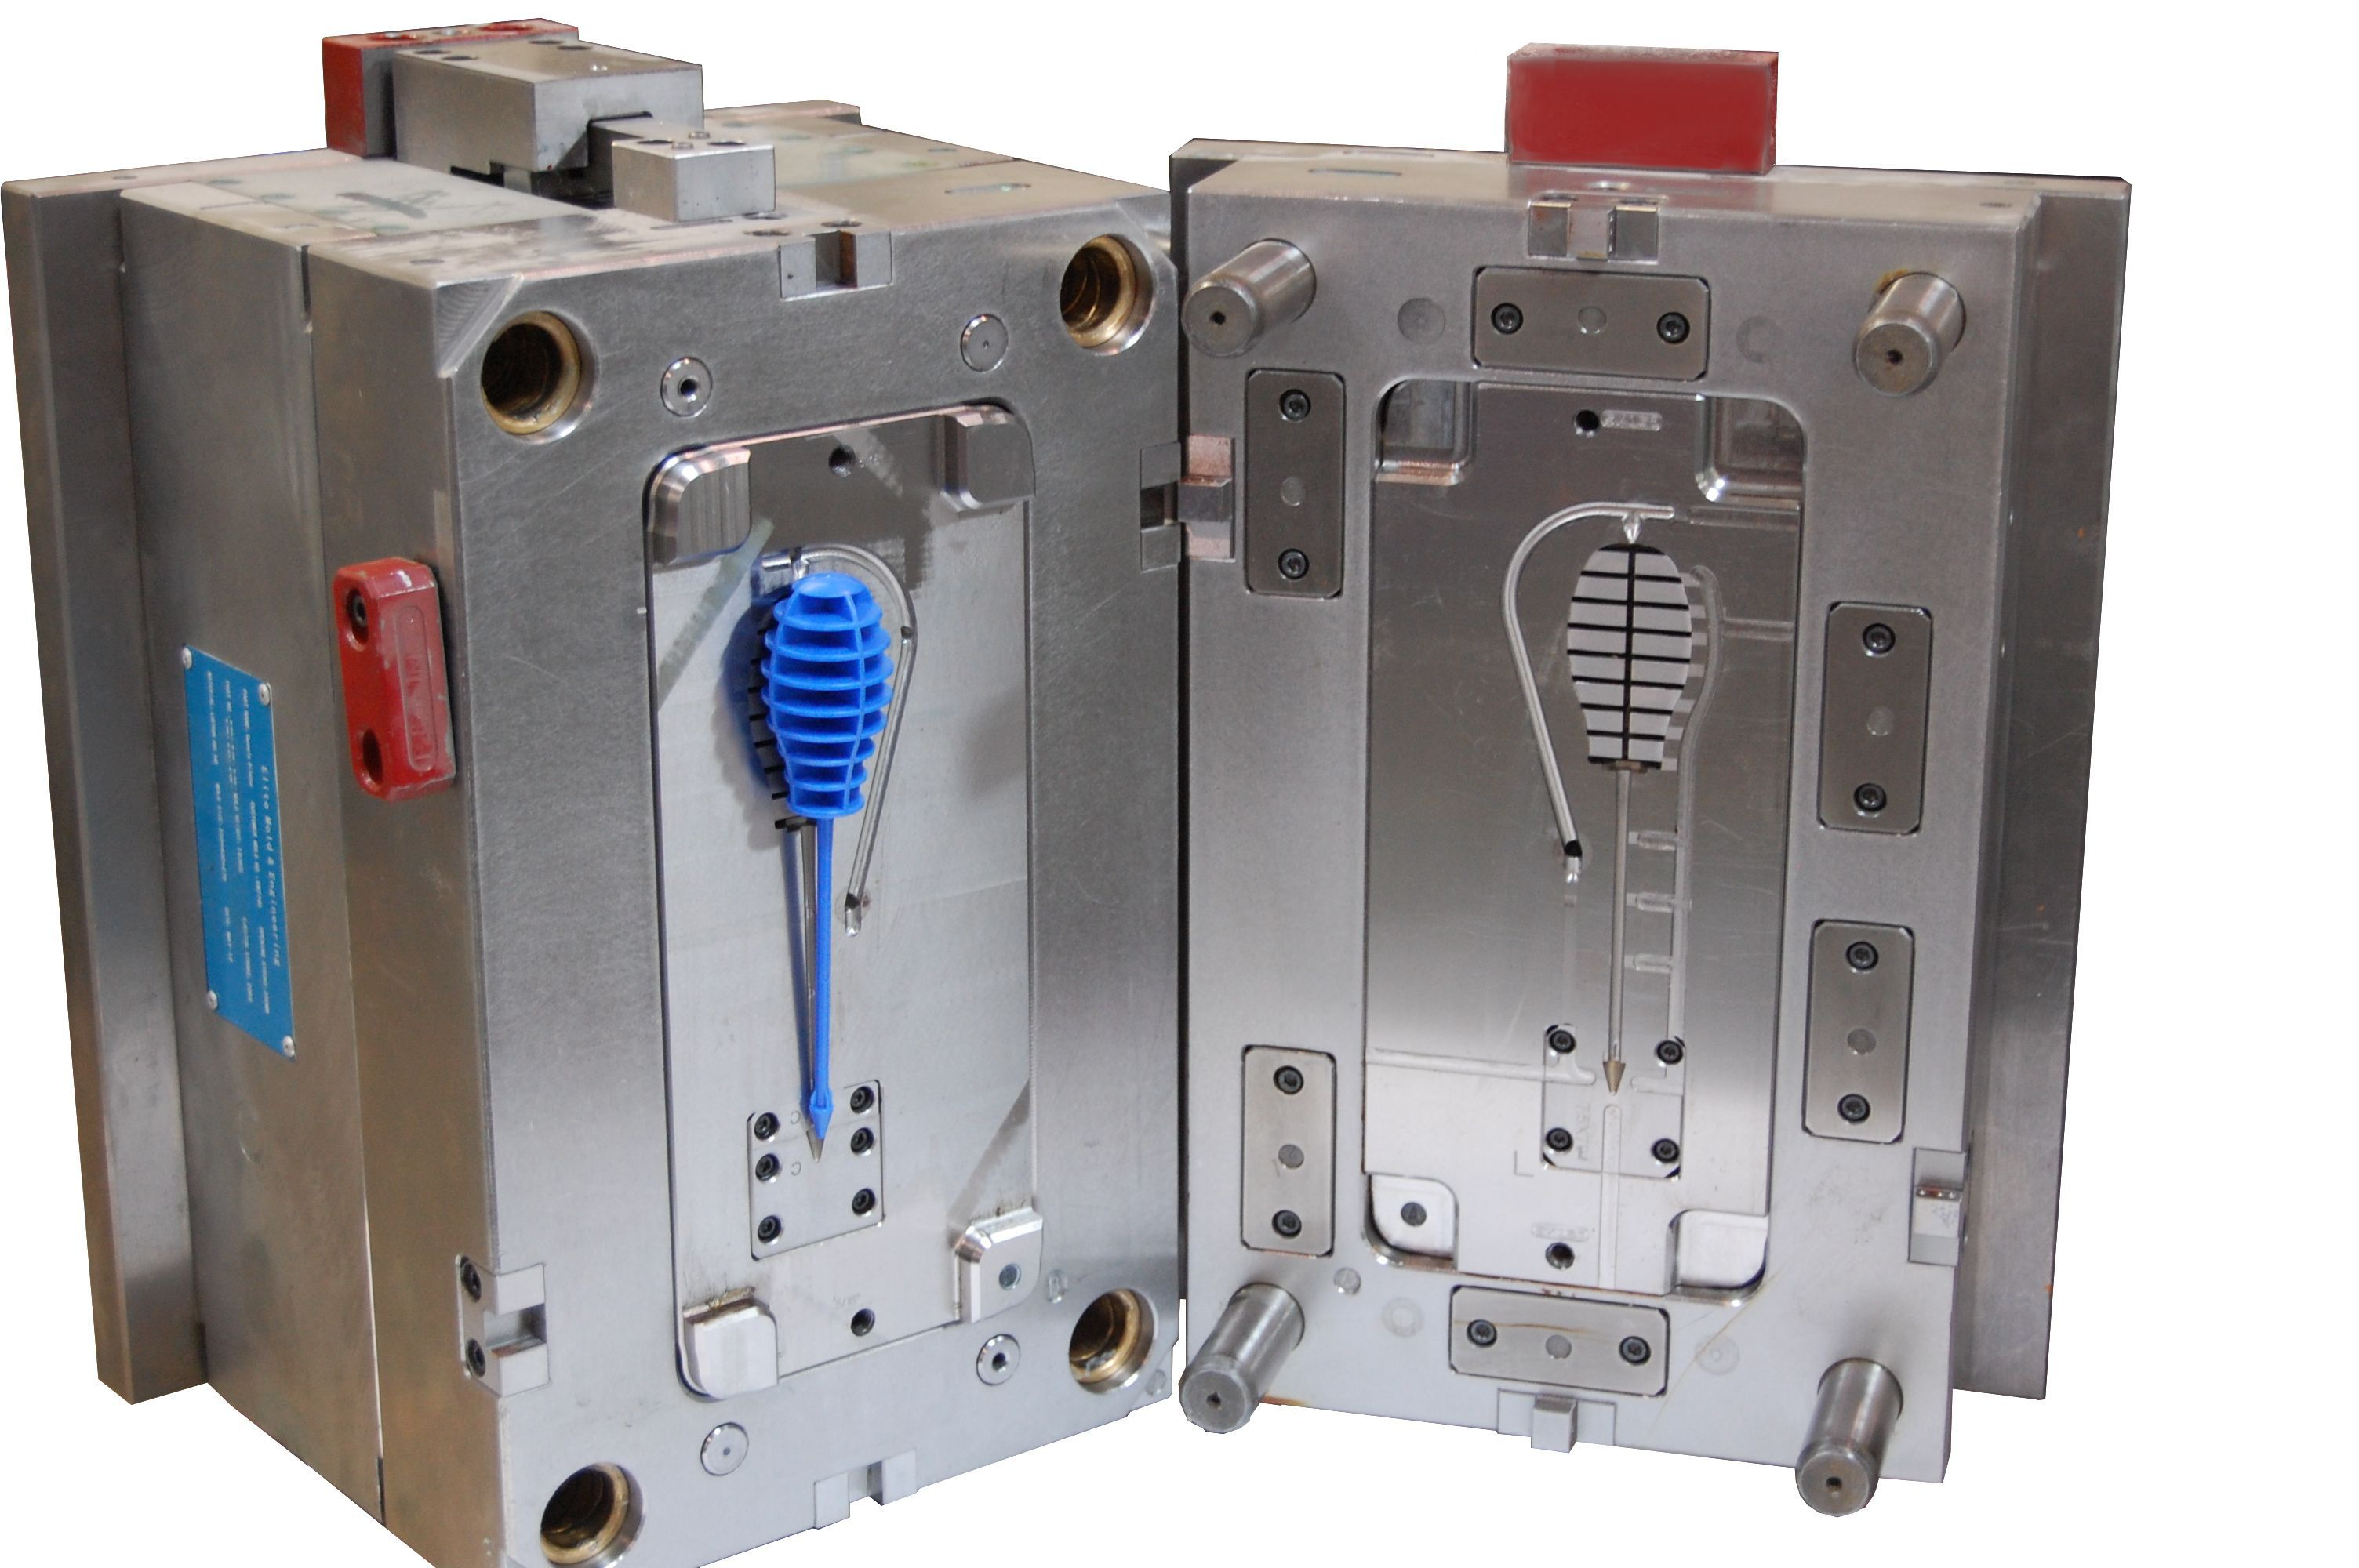
\includegraphics[width=0.9\textwidth]{molde} % Include the image placeholder.png
		\caption{Molde}
		\label{fig:molde}
	\end{center}
\end{figure}
Moldagem é o processo mecânico de dar forma a um material no estado líquido usando um molde\cite{definicao_moldagem,definicao_moldar}. Um molde é uma ferramenta sólida oca desenvolvida para efeitos de fundição\cite{definicao_molde}. Esta é enchida com um material em estado liquido ou em pó como plástico, metal, cerâmica ou vidro\cite{Williams1975,Trovant1998,JanneyMarkA.Knoxville1991,Yan2009}.\par
A moldagem por injeção é particularmente útil na produção em massa de peças de plástico com elevada complexidade geométrica\cite{Shen,Shelesh}. Estas podem ser encontradas em todas as áreas da industria como por exemplo empacotamento, aviação, construção e eletrónica\cite{Ozcelik}. Neste processo, plástico quente é forçado para dentro de um molde frio com a forma desejada. O material cobre todas as feições do molde e vai endurecendo sobre o efeito de altas pressões. O processo de injeção pode ser divido em fases distintas\cite{Shen}:
\begin{itemize}[noitemsep]
	\item Fecho do molde
	\item Enchimento
	\item Compactação
	\item Abertura do molde
	\item Extração
\end{itemize}
Em 1868, John Wesley Hyatt inventou uma maneira de fazer bolas de bilhar injetando celuloide para dentro de um molde\cite{historia,patente1868}.\par
Em 1872 Jonh e o seu irmão Isaiah patentearam a primeira máquina de moldes de injeção. Esta era relativamente simples comparada às que são usadas hoje em dia na indústria. Consistia de um pequeno embolo para injetar plástico num molde através de um cilindro quente\cite{historia,patente1872}.\par
A indústria cresceu lentamente produzindo artigos de plástico como botões e pentes. Nos anos 40 a utilização de moldes de injeção cresceu por causa da Segunda Guerra Mundial que tinha uma grande procura de produtos baratos e produzidos em massa\cite{historia}.\par
Em 1946, James Hendry construiu a primeira máquina de moldes de injeção com um sem fim, revolucionando a indústria dos plásticos com um design para substituir o embolo de Hyatt. Este sem fim é colocado dentro do cilindro e mistura o material a ser moldado antes de ser injetado no molde. Isto permitiu que cor ou plástico reciclado fossem adicionados à mistura\cite{historia,patente1946}.\par
A indústria do moldes de injeção evoluiu bastante sendo desenvolvidos vários métodos de otimização, desde processos mecânicos a processos de monitorização por computador. Neste projeto é dado mais um passo no campo da monitorização remota de moldes, criando um histórico destes para efeitos de análise.\par


\section{base de dados relacional}

\section{SQL}

\section{internet tcp/ip}

\section{Software utilizado}
\subsection{Linux}

\subsection{MySQL}

\subsection{C}

\subsection{Apache}

\subsection{PHP e HTML}

\cleardoublepage
\chapter{Proposta de Solução}
\section{Infraestrutura de dados}

\section{Base de Dados}
\subsection{Análise de Requisitos}

\subsection{Desenho conceptual e esquema lógico}

\subsection{Construção da base de dados}

\subsection{Programa de transferência}

\subsection{Gestão de \textit{backups}}
\label{subchap:backups}

\subsection{Simulador}

\subsection{Utilizadores}

\cleardoublepage
\chapter{Aplicação}
Aplicação desenvolvida em ambiente  \textit{Web} com o objetivo de ser multiplataforma, permitir acesso remoto e sem recorrer a instalação de \textit{softwares} nos dispositivos dos utilizadores. Esta corre num servidor \textit{Apache} e foi desenvolvida com \textit{PHP} e \textit{HTML}. Este capítulo descreve a adaptação da infraestrutura desenvolvida e as várias funcionalidades da aplicação.

\section{Adaptação da infraestrutura}
Afim de garantir uma maior integridade dos dados inseridos pela aplicação, instala-se no servidor local uma nova base de dados temporária local. Aqui os utilizadores têm a liberdade para adicionar, alterar e apagar informação sem consequências no sistema antes destas serem introduzidas nas bases de dados central e local como representado na \autoref{fig:adap1}. Como referido anteriormente, esta base de dados difere das restantes, não contendo em si as tabelas fase e registos.
\begin{figure}[H]
	\begin{center}
		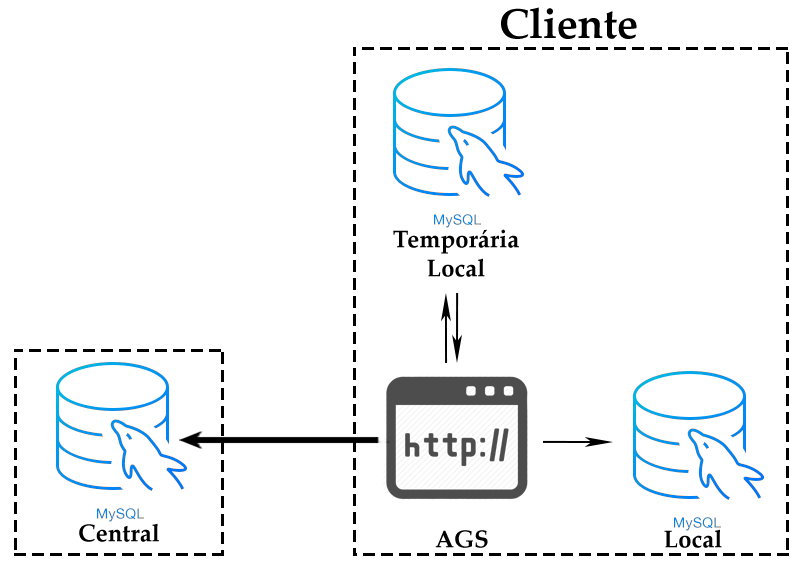
\includegraphics[width=0.65\textwidth]{Aplicacao_temp_local_central} % Include the image placeholder.png
		\caption{Esquema ligação Aplicação-bases de dados. A aplicação comunica com a base de dados temporária local e depois regista os valores desta nas bases de dados central e local}
		\label{fig:adap1}
	\end{center}
\end{figure}

\section{Interface gráfica}
A aplicação divide-se em cinco partes distintas:
\begin{itemize}[noitemsep]
	\item \textit{Main}
	\item \textit{Login}
	\item Consultas
	\item Administração
	\item Conexão Local
\end{itemize}
As páginas \textit{Main}, \textit{Login}, Consultas e parte das funcionalidades da Administração foram realizadas para uma utilização geral. As páginas Conexão Local e as restantes funcionalidades da Administração foram realizadas para uma utilização local. A primeira visa um uso a partir de qualquer dispositivo e acessível a qualquer momento e a segunda foca-se num acesso local com o objetivo de configurar e definir a informação no servidor local. Por outras palavras, para o utilizador usar as funcionalidades destas páginas tem de aceder à aplicação no sistema local que se situa no cliente.\\
Instalar um molde é culminar de um projeto de elevada responsabilidade, esta ideia junto com a criação da base de dados temporária local serve para melhorar a qualidade da informação introduzida no sistema e diminuir as falhas.\\

\newpage
\subsection{\textit{Main}}
\begin{figure}[H]
\centering
	\begin{minipage}{1.\textwidth}
		\begin{center}
			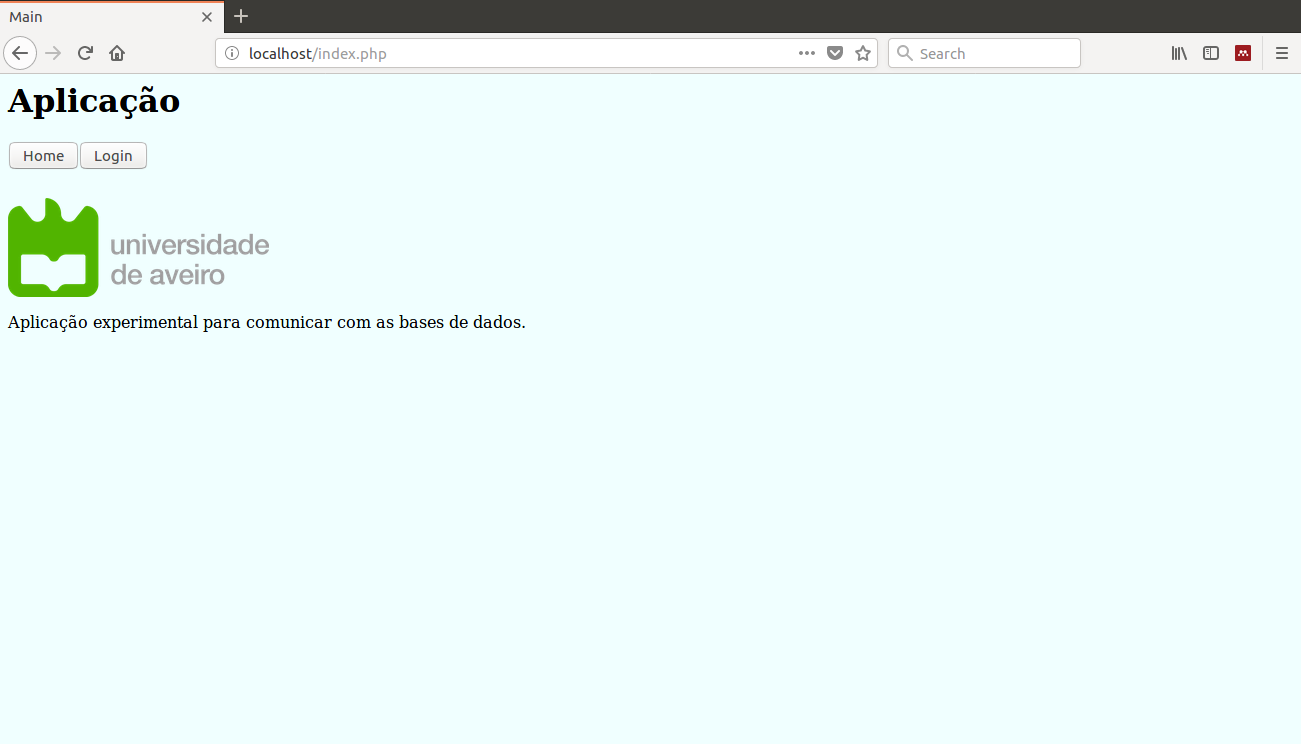
\includegraphics[width=0.85\textwidth]{main01} % Include the image placeholder.png
			\subcaption{Sem \textit{login}}
			\label{fig:main1}
		\end{center}
	\end{minipage}
	\begin{minipage}{1.\textwidth}
		\begin{center}
			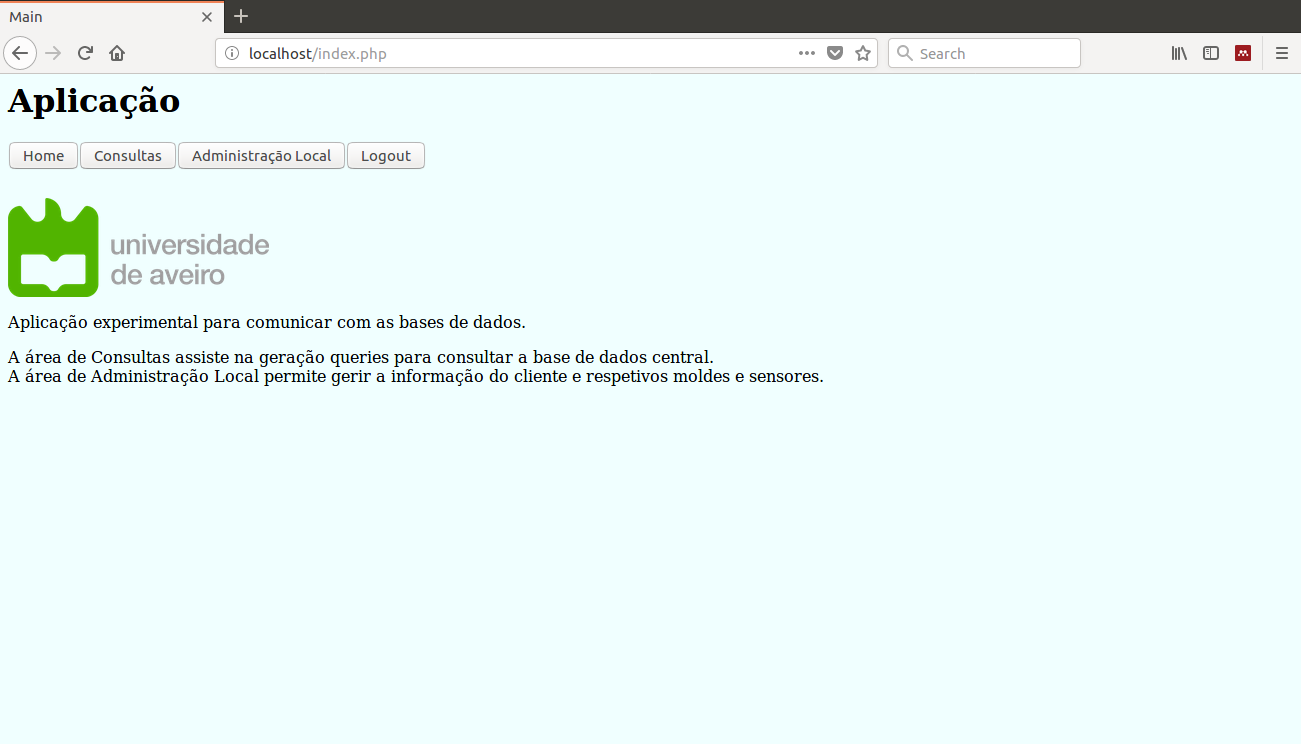
\includegraphics[width=0.85\textwidth]{main02} % Include the image placeholder.png
			\subcaption{Com \textit{login}}
			\label{fig:main2}
		\end{center}
	\end{minipage}
	\caption{Funcionalidades da página \textit{Main} com e sem \textit{login}}
	\label{fig:main0}
\end{figure}
\textit{Main} serve como página principal da aplicação. Se não houver sessão iniciada todas as restantes páginas redirecionam o utilizador para aqui. Contém apenas algumas informações gerais sobre a aplicação.\\
Iniciar sessão na página de \textit{Login} desbloqueia funcionalidades na aplicação, como demonstrado nas Figuras \ref{fig:main1} e \ref{fig:main2}. Depois de iniciada sessão navega-se com os botões para as páginas de Consultas, Administração e Conexão Local.

\subsection{\textit{Login}}
\begin{figure}[H]
	\begin{center}
		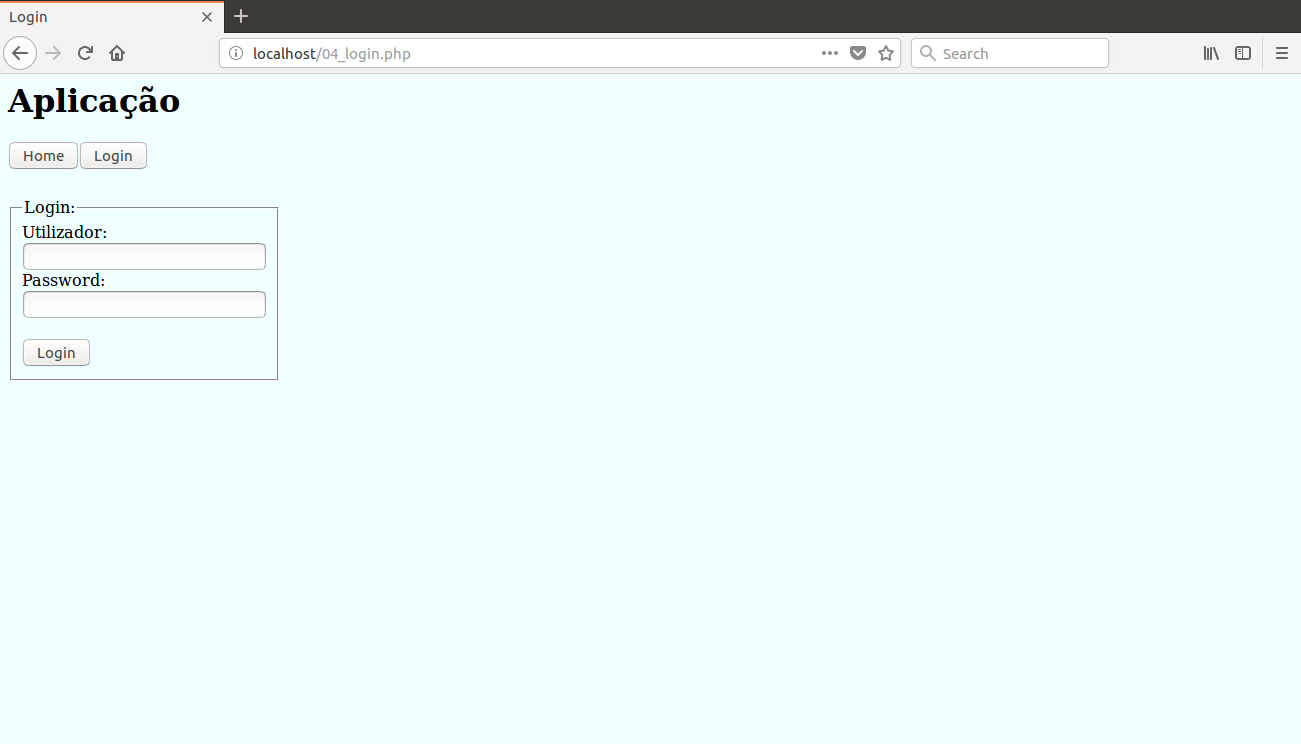
\includegraphics[width=0.9\textwidth]{login01} % Include the image placeholder.png
		\caption{Página de \textit{Login} para iniciar sessão na base de dados central}
		\label{fig:login0}
	\end{center}
\end{figure}
A página de \textit{Login} consiste num simples formulário constituído por duas caixas de texto e um botão, como demonstrado na \autoref*{fig:login0}. O botão \textit{Login} lê as credenciais introduzidas e realiza uma conexão de teste à base de dados central validando-as diretamente com \textit{MySQL}. Se as credenciais forem validadas com sucesso redireciona-se o utilizador para a página principal e altera-se o botão de \textit{Login} para \textit{Logout}. Se as credenciais introduzidas não forem suficientes ou válidas são retornados erros de forma a informar o utilizador como demonstrado nas Figuras \ref{fig:login2} e \ref{fig:login3}.\\
Quando se acede à página como \textit{Logout} termina-se a sessão e redireciona-se o utilizador para a página principal.
\begin{figure}[H]
	\centering
	\begin{minipage}{.5\textwidth}
		\begin{center}
			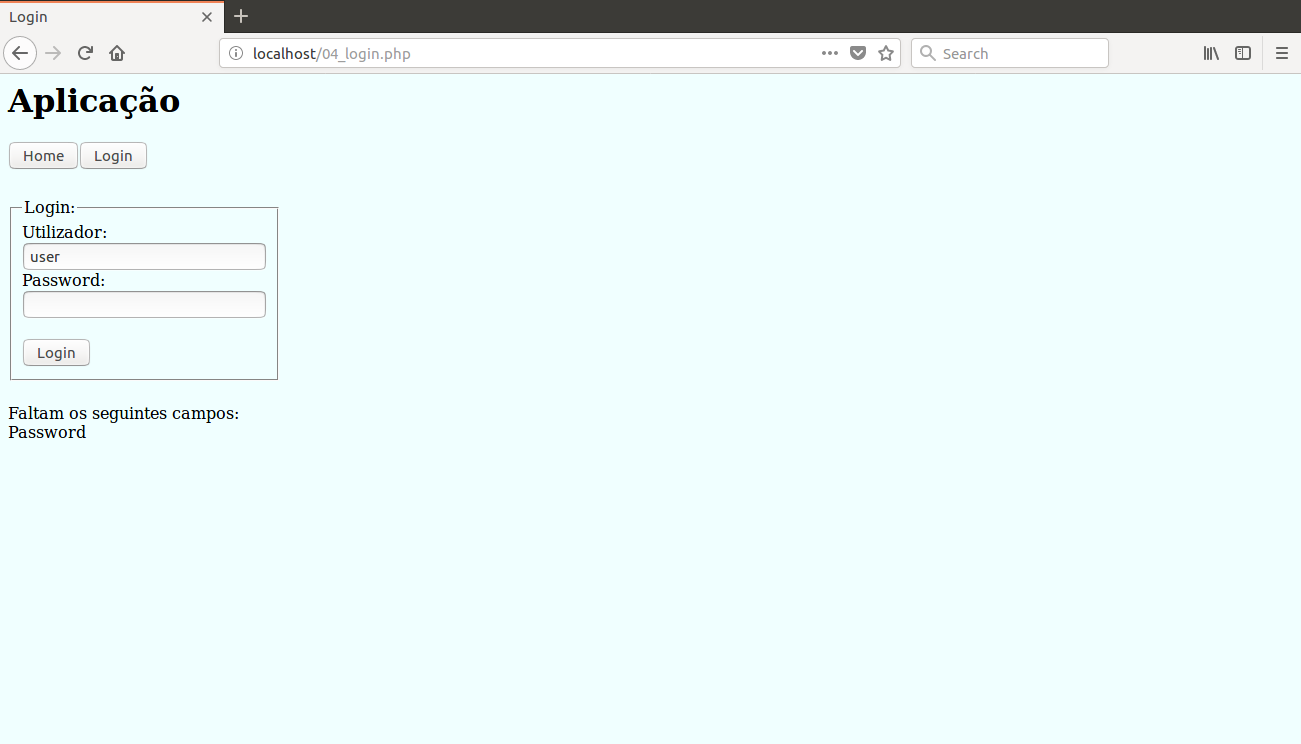
\includegraphics[width=0.95\textwidth]{login02} % Include the image placeholder.png
			\subcaption{Exemplo de erro de falta de informação}
			\label{fig:login2}
		\end{center}
	\end{minipage}%
	\begin{minipage}{.5\textwidth}
		\begin{center}
			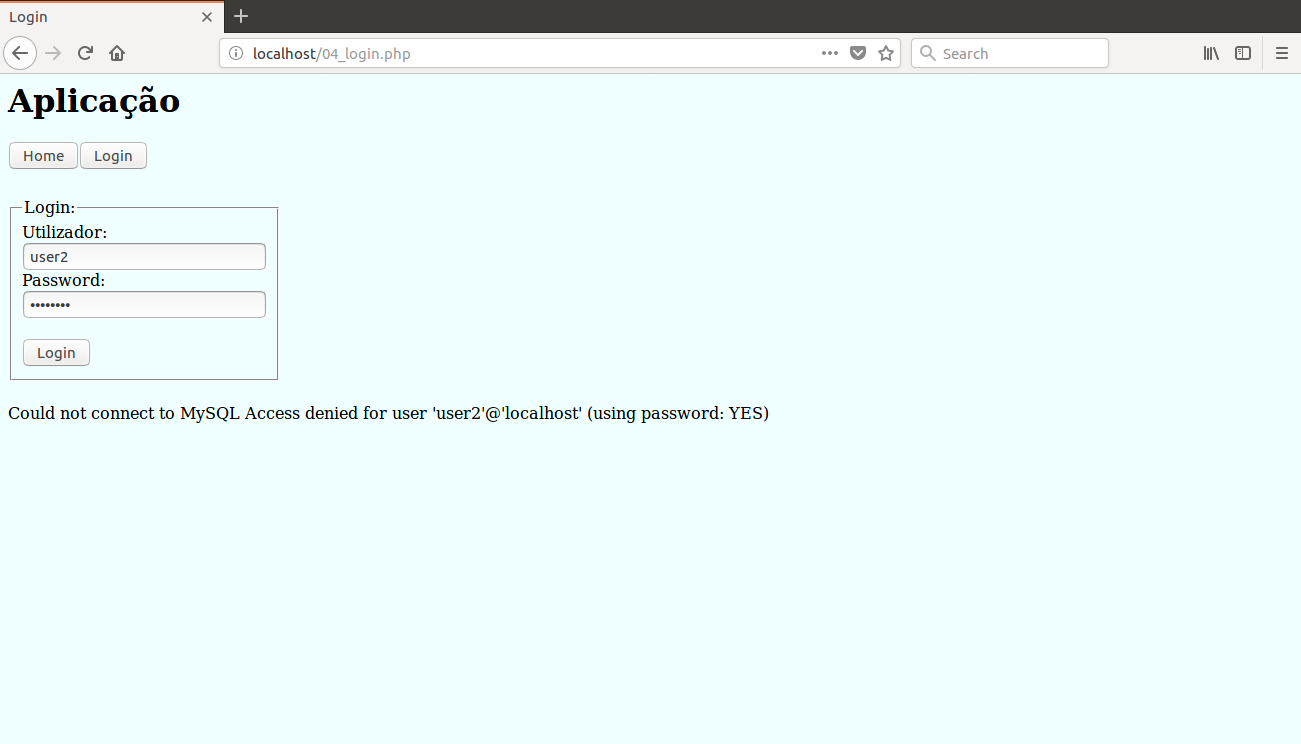
\includegraphics[width=0.95\textwidth]{login03} % Include the image placeholder.png
			\subcaption{Exemplo de erro \textit{MySQL}}
			\label{fig:login3}
		\end{center}
	\end{minipage}
	\caption{Exemplos de erros retornados quando introduzidas credenciais não válidas na página \textit{Login}}
	\label{fig:login1}
\end{figure}

\subsection{Consultas}
\begin{figure}[H]
	\centering
	\begin{minipage}{1.\textwidth}
		\begin{center}
			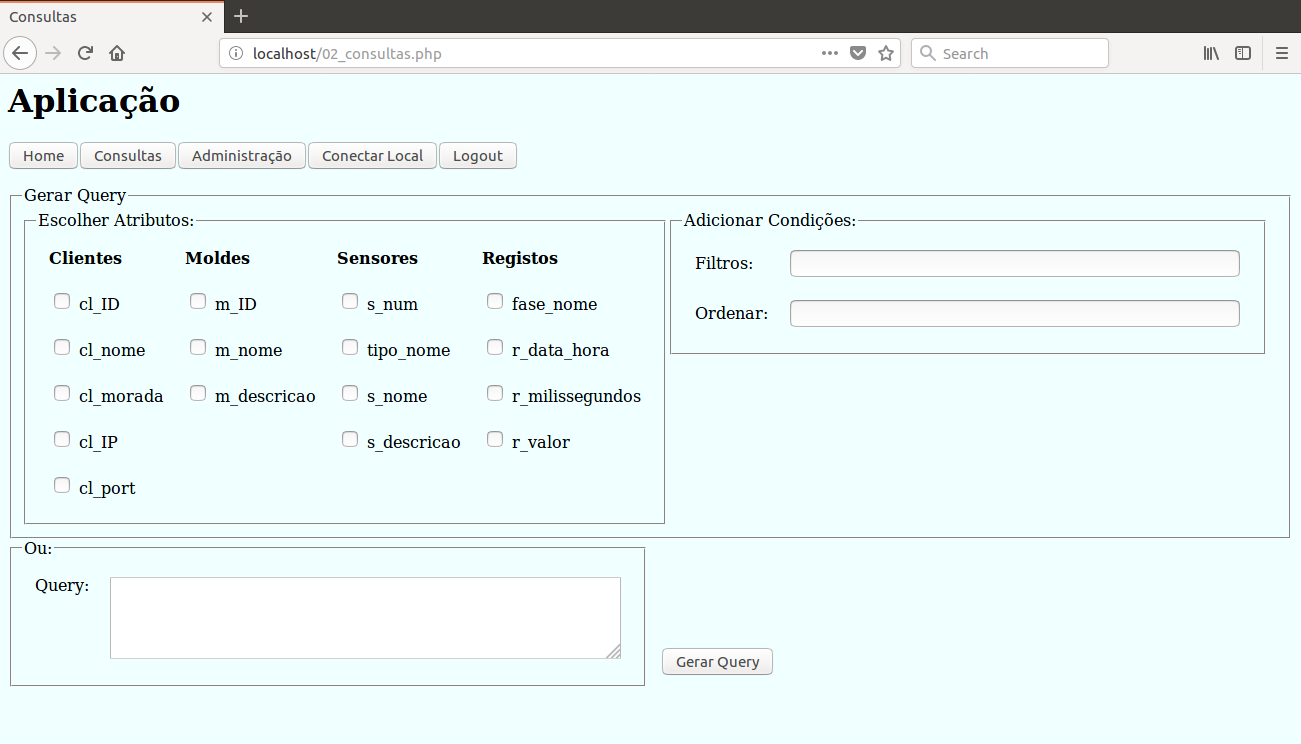
\includegraphics[width=.9\textwidth]{consultas01} % Include the image placeholder.png
			\subcaption{Página de Consultas}
			\label{fig:consultas1}
		\end{center}
	\end{minipage}
	\begin{minipage}{1.\textwidth}
		\begin{center}
			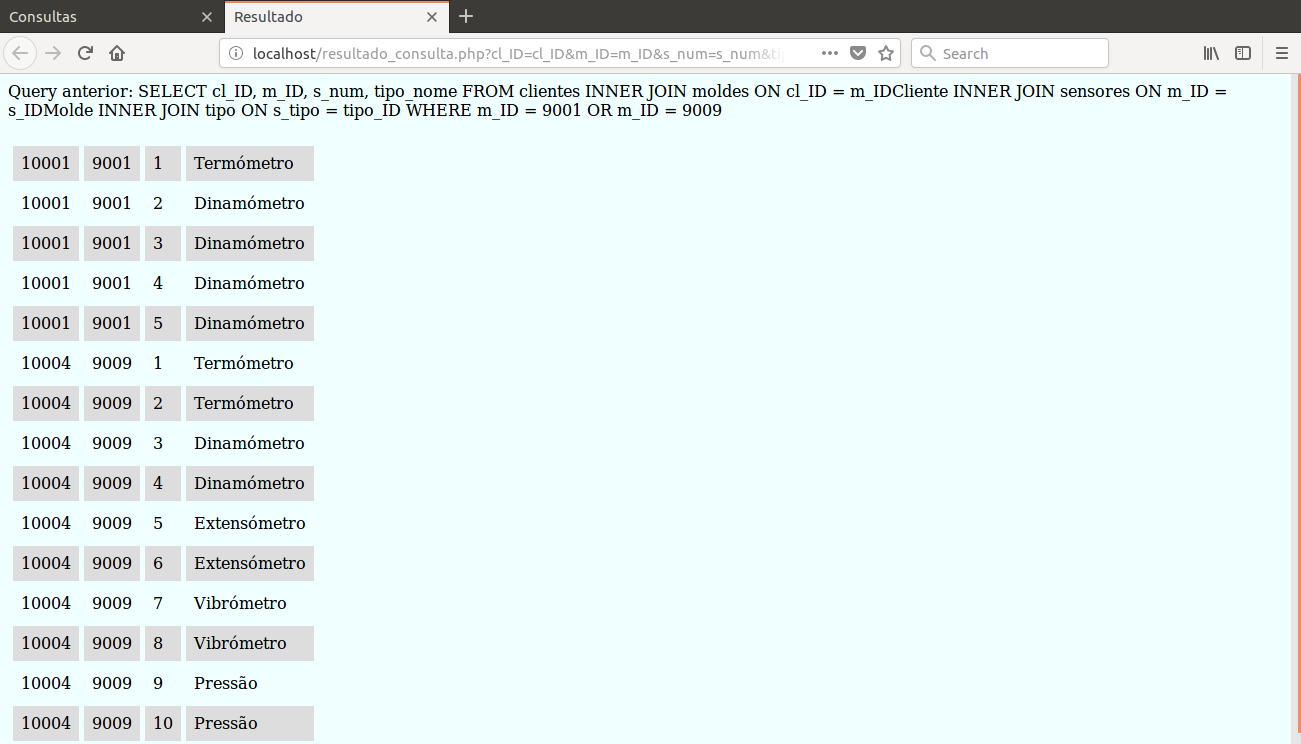
\includegraphics[width=0.9\textwidth]{consultas02} % Include the image placeholder.png
			\subcaption{Exemplo de resposta de consulta}
			\label{fig:consultas2}
		\end{center}
	\end{minipage}
	\caption{Página de Consultas e exemplo de resposta a uma consulta}
	\label{fig:consultas0}
\end{figure}
A página de Consultas assiste utilizadores sem conhecimentos de \textit{SQL} a criarem \textit{queries} para consultar a base de dados central. Na \autoref{fig:consultas1} observa-se várias \textit{checkboxes} e três caixas de texto. As \textit{checkboxes} permitem selecionar os atributos que se desejam consultar na base de dados, estes são guardados numa variável @atributos.
\newpage
Quando  se prime o botão \textit{Query} gera-se uma das seguintes \textit{queries}:\\
\begin{lstlisting}[language = SQL]
	SELECT @atributos
	FROM clientes;
	
	SELECT @atributos
	FROM clientes
	INNER JOIN moldes ON cl_ID = m_IDCliente;
	
	SELECT @atributos
	FROM clientes
	INNER JOIN moldes ON cl_ID = m_IDCliente
	INNER JOIN sensores ON m_ID = s_IDMolde
	INNER JOIN tipo ON s_tipo = tipo_ID;
	
	SELECT @atributos FROM clientes
	INNER JOIN moldes ON cl_ID = m_IDCliente
	INNER JOIN sensores ON m_ID = s_IDMolde 
	INNER JOIN tipo ON s_tipo = tipo_ID
	INNER JOIN registos ON s_IDMolde = r_IDMolde
	AND s_num = r_numSensor
	INNER JOIN fase ON r_fase = fase_ID;
\end{lstlisting}
Efetua-se esta seleção com base na coluna mais à esquerda a que os atributos pertencem. Explicando melhor com um exemplo: se o utilizador desejar consultar o cl\texttt{\char`_}ID e o cl\texttt{\char`_}nome da tabela clientes gera-se a primeira \textit{query} no entanto, se o utilizador desejar consultar os atributos cl\texttt{\char`_}ID, m\texttt{\char`_}ID e s\texttt{\char`_}num gera-se a terceira \textit{query}.\\
Além destas, existem três \textit{queries} especificas quando os atributos tipo\texttt{\char`_}nome, fase\texttt{\char`_}nome e r\texttt{\char`_}data\texttt{\char`_}hora são selecionados sozinhos. As primeiras duas permitem consultar as opções disponíveis nos dicionários e a terceira devolve as datas e horas entre o primeiro e último registos.\\
As caixas de texto Filtros e Ordem permitem adicionar às \textit{queries} geradas as cláusulas WHERE e ORDER BY, respetivamente. Para os utilizadores com conhecimentos em \textit{SQL} está disponibilizada a caixa de texto \textit{Query} que permite a criação direta de uma \textit{query}. Este campo está limitado apenas para \textit{queries} do tipo SELECT.\\
Depois da \textit{query} ser gerada retorna-se uma resposta num novo separador como demonstrado na \autoref{fig:consultas2}. O \textit{link} deste resposta contém toda a informação da \textit{query} gerada. Este pode ser arquivado ou enviado para outro utilizador sem ser necessário gerar a \textit{query} novamente, isto é útil para \textit{queries} com muitas cláusulas.\\
Se a \textit{query} não for válida retorna-se um erro de forma a informar o utilizador, como demonstrado nas Figuras \ref{fig:consultas4}, \ref{fig:consultas5} e \ref{fig:consultas6}.
\newpage
\begin{figure}[H]
	\centering
	\begin{minipage}{1\textwidth}
		\begin{center}
			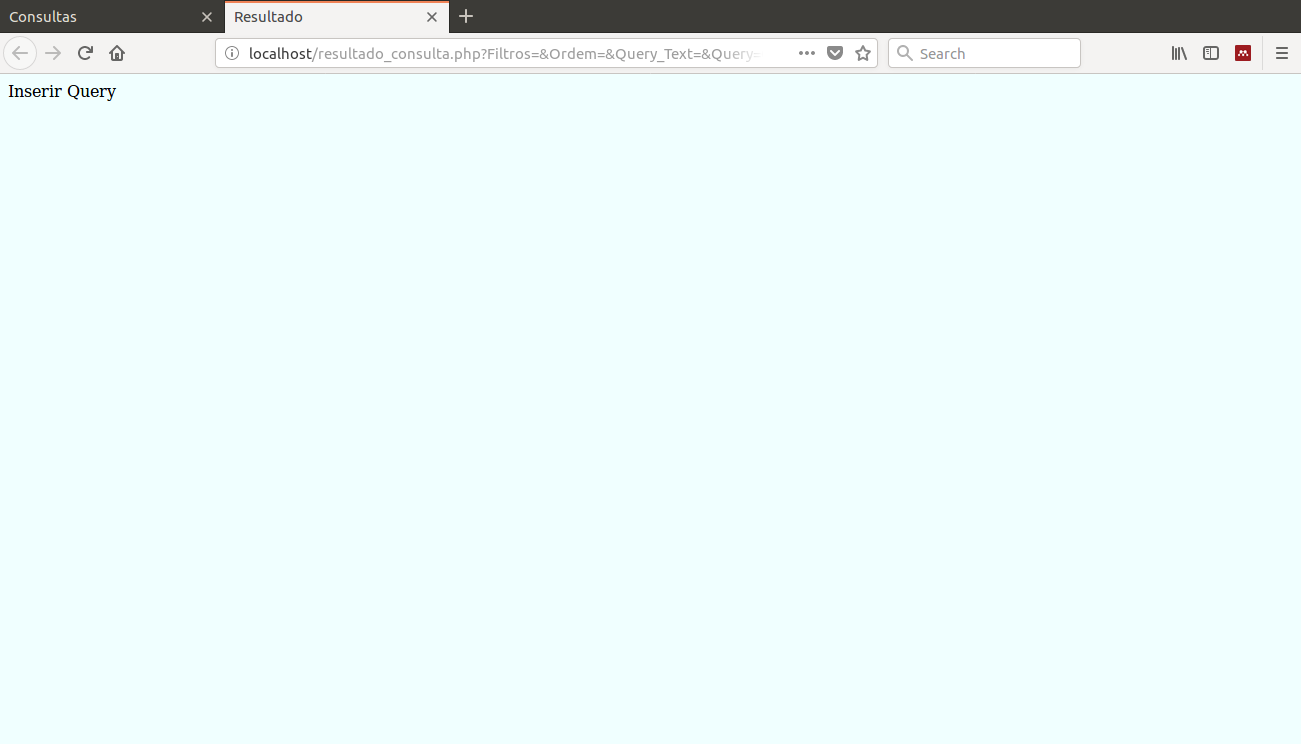
\includegraphics[width=0.7\textwidth]{consultas03} % Include the image placeholder.png
			\subcaption{Erro de informação não introduzida}
			\label{fig:consultas4}
		\end{center}
	\end{minipage}
	\begin{minipage}{1\textwidth}
		\begin{center}
			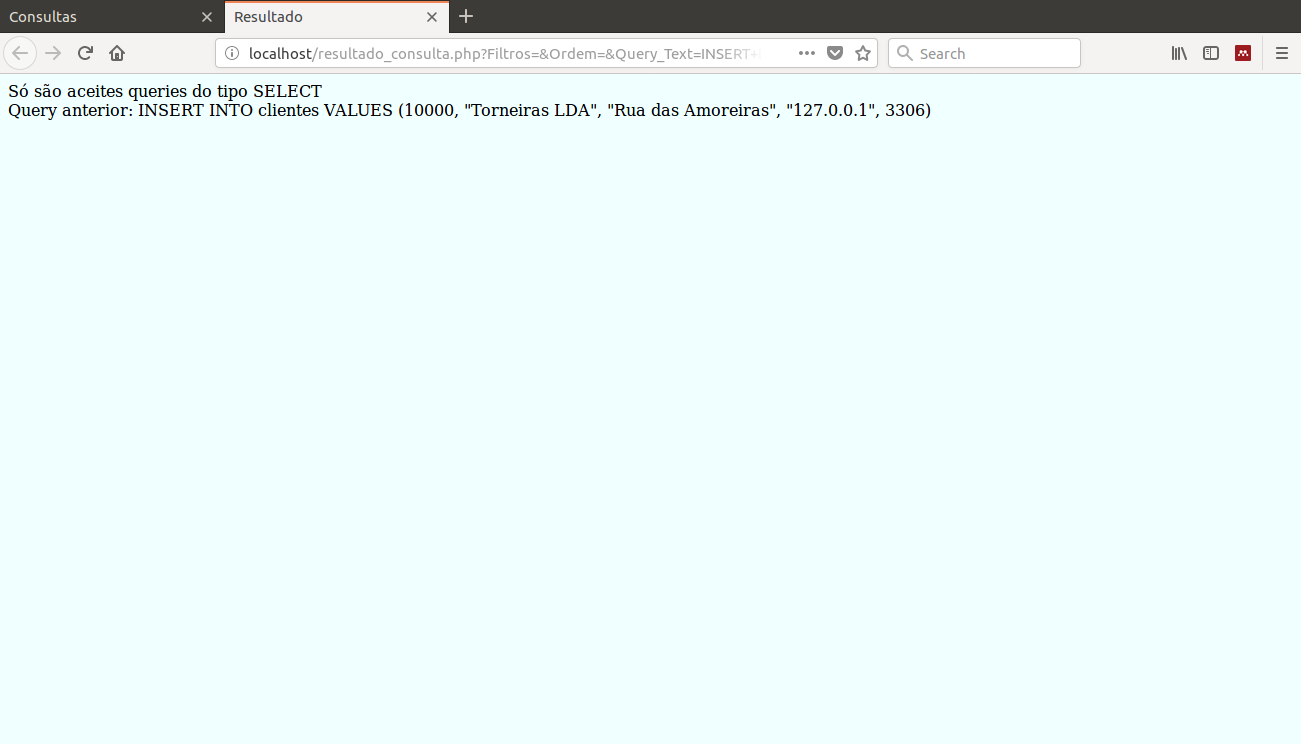
\includegraphics[width=0.7\textwidth]{consultas04} % Include the image placeholder.png
			\subcaption{Erro de \textit{query} que não é do tipo SELECT}
			\label{fig:consultas5}
		\end{center}
	\end{minipage}
	\begin{minipage}{1\textwidth}
		\begin{center}
			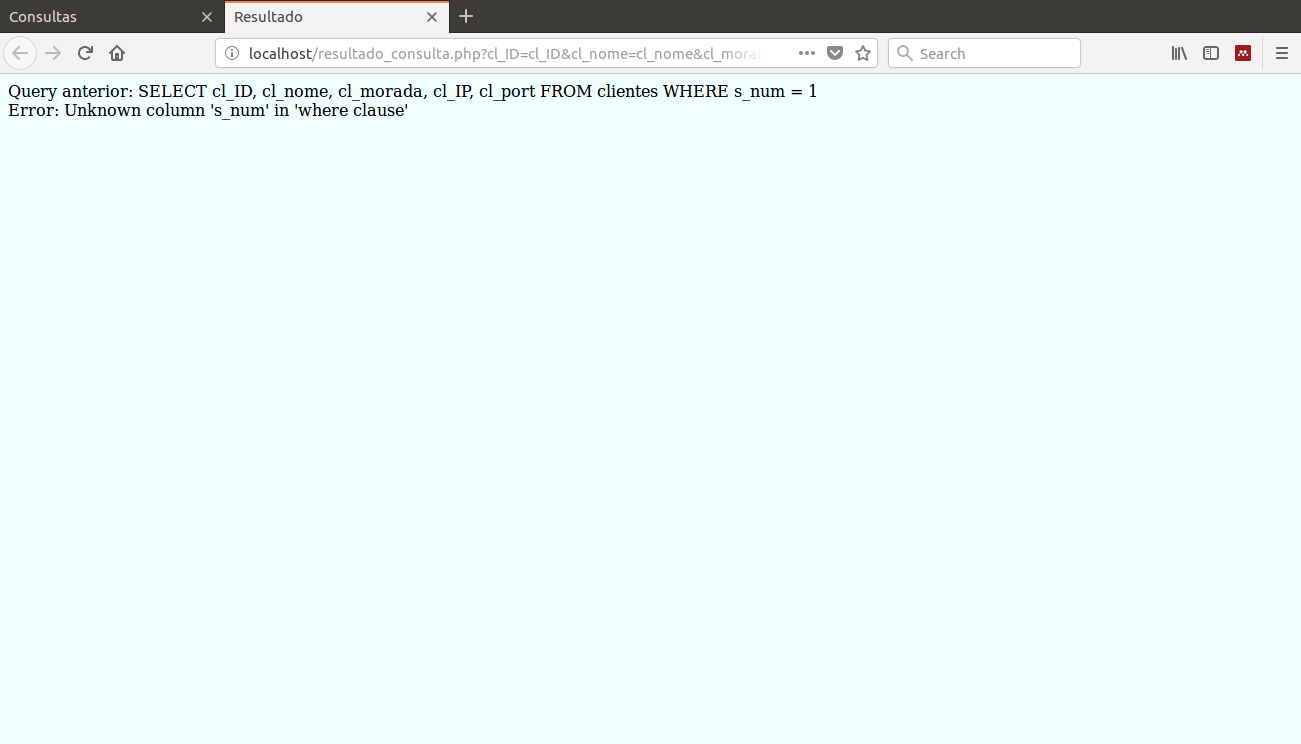
\includegraphics[width=0.7\textwidth]{consultas05} % Include the image placeholder.png
			\subcaption{Exemplo de erro \textit{MySQL}}
			\label{fig:consultas6}
		\end{center}
	\end{minipage}
	\caption{Exemplos de erros retornados na página de Resposta da Consulta}
	\label{fig:consultas3}
\end{figure}

\subsection{Administração}
\begin{figure}[H]
	\centering
	\begin{minipage}{1\textwidth}
		\begin{center}
			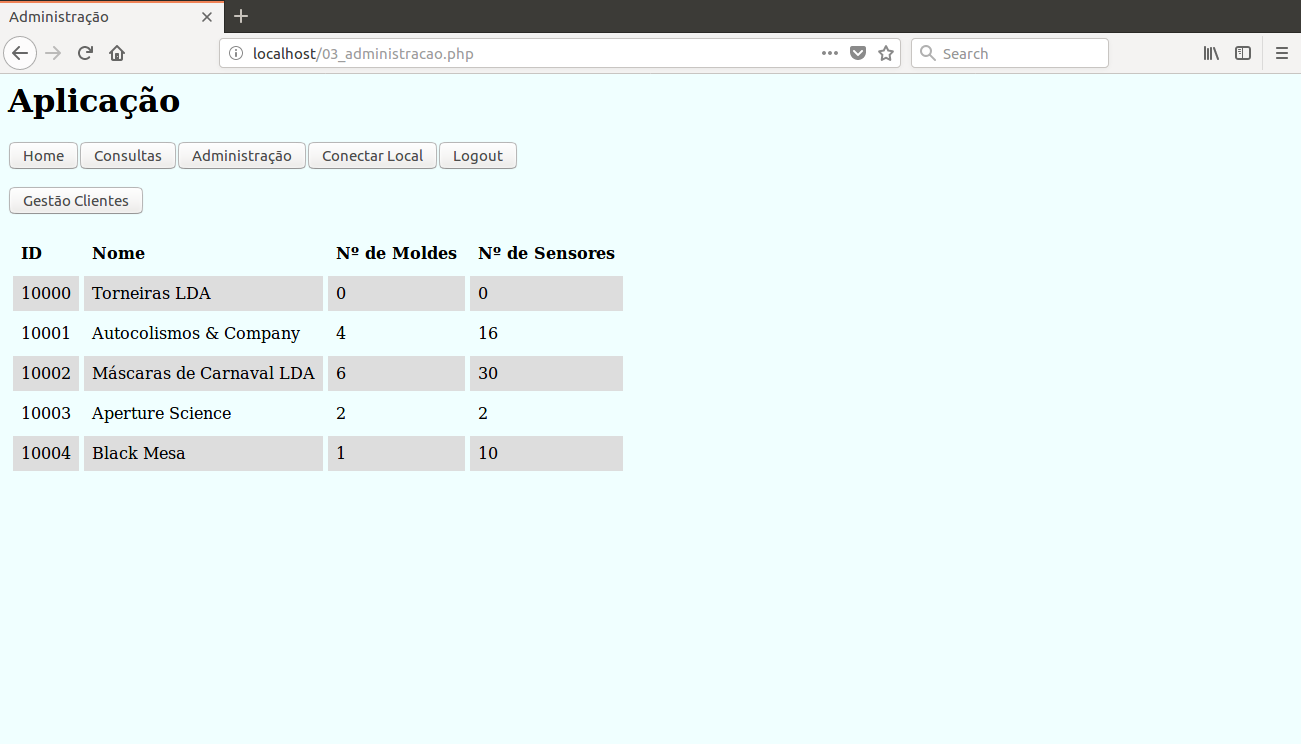
\includegraphics[width=0.9\textwidth]{administracao01} % Include the image placeholder.png
			\subcaption{Sem conexão local}
			\label{fig:admin1}
		\end{center}
	\end{minipage}
	\begin{minipage}{1\textwidth}
		\begin{center}
			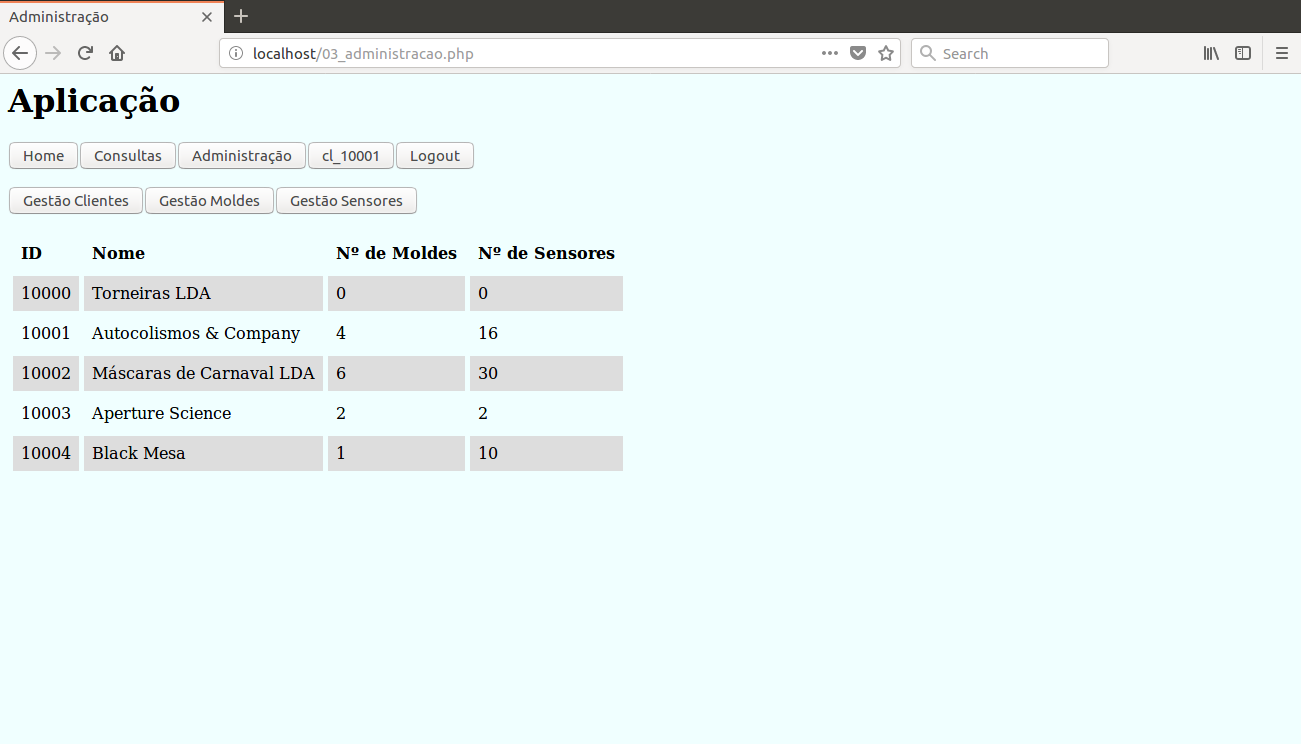
\includegraphics[width=0.9\textwidth]{administracao03} % Include the image placeholder.png
			\subcaption{Com conexão local}
			\label{fig:admin2}
		\end{center}
	\end{minipage}
	\caption{Funcionalidades da página Administração com e sem conexão local}
	\label{fig:admin0}
\end{figure}
\newpage
A área de Administração permite ao utilizador alterar informações sobre os clientes, moldes e sensores. A partir de qualquer dispositivo só é possível aceder à Gestão de Clientes como demonstrado na \autoref{fig:admin1}. Nesta área a informação dos clientes pode ser alterada com o formulário demonstrado na \autoref{fig:admin3}. Os botões Adicionar Cliente, Alterar Cliente e Eliminar Cliente executam \textit{queries} do tipo INSERT, UPDATE e DELETE, respetivamente.\\
\\
\\
\\
\\
\\
\\
\\
\\
\\
\\
\begin{figure}[H]
	\begin{center}
		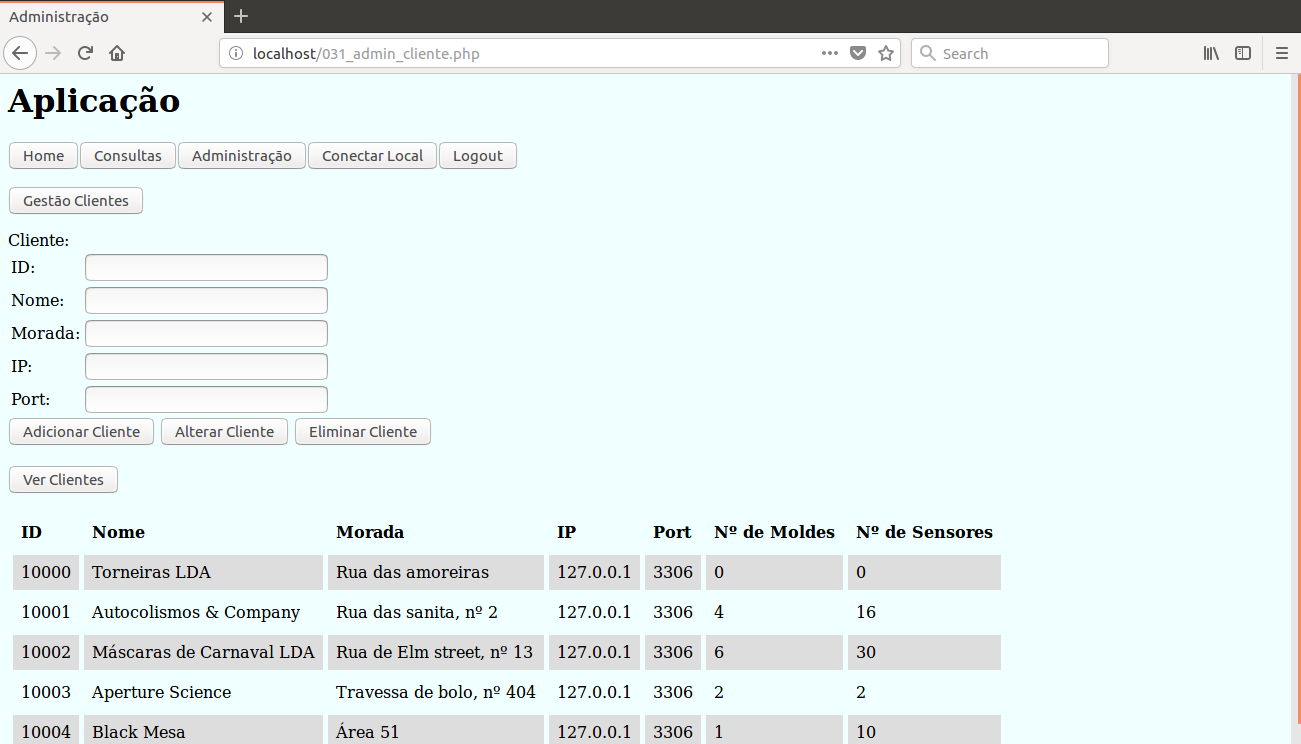
\includegraphics[width=0.9\textwidth]{administracao02} % Include the image placeholder.png
		\caption{Área de Gestão de Clientes sem conexão local}
		\label{fig:admin3}
	\end{center}
\end{figure}
\newpage
Como referido anteriormente a aplicação divide-se numa utilização geral e local, todas as funcionalidades descritas até agora têm em vista uma utilização geral. As restantes funcionalidades que são descritas até ao final do capítulo visam um uso local.\\
Após uma conexão bem sucedida ao sistema local do cliente são desbloqueadas novas áreas de gestão como mostra a \autoref{fig:admin2}. As áreas de Gestão de Moldes e Gestão de Sensores demonstradas nas Figuras \ref{fig:admin9} e \ref{fig:admin10}, permitem ao utilizador criar e apagar moldes e sensores, respetivamente. Estes dados são inseridos na base de dados temporária local, aqui o utilizador pode criar e apagar moldes e sensores sem afetar o sistema. Desta forma é possível confirmar a informação introduzida antes de a inserir no sistema. Os botões de Criar e Apagar nestes formulários realizam \textit{queries} do tipo INSERT e DELETE, respetivamente.
	\begin{figure}[H]
		\centering
			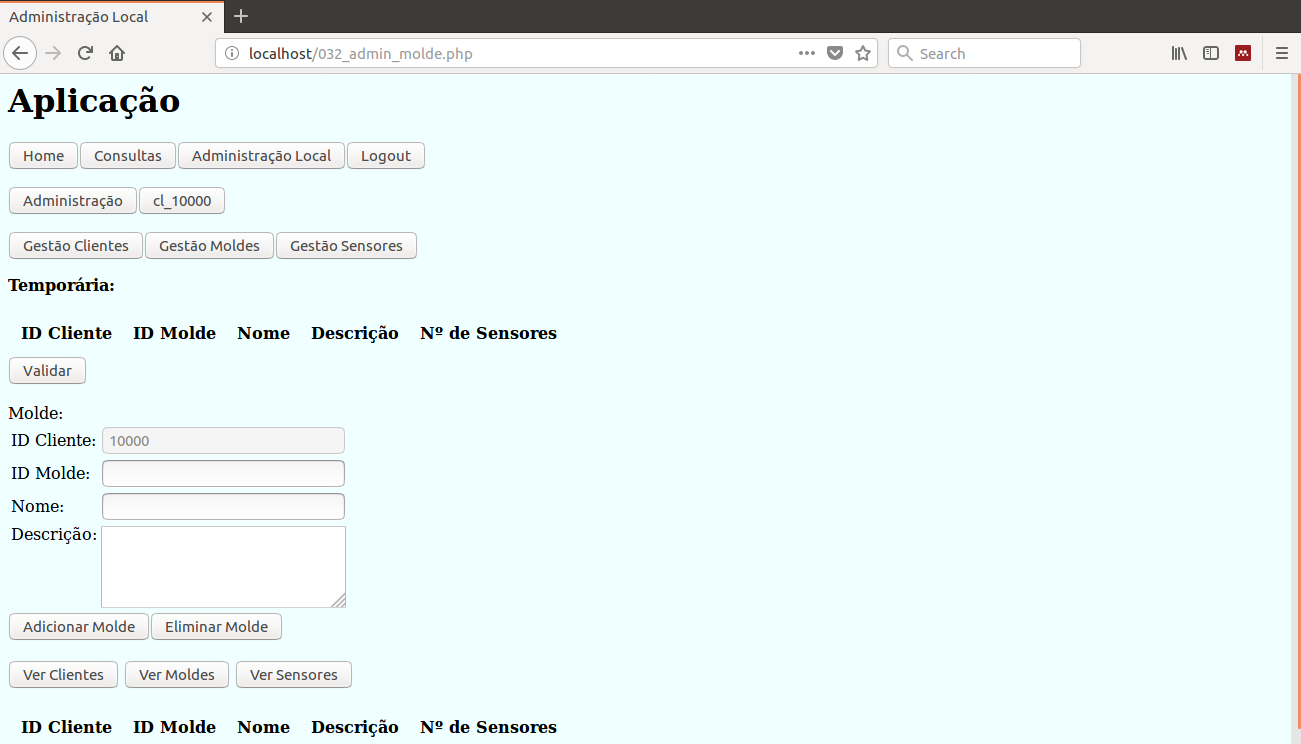
\includegraphics[width=0.8\textwidth]{administracao05} % Include the image placeholder.png
			\caption{Área de Gestão de Moldes}
			\label{fig:admin9}
	\end{figure}
	\begin{figure}[H]
		\centering
			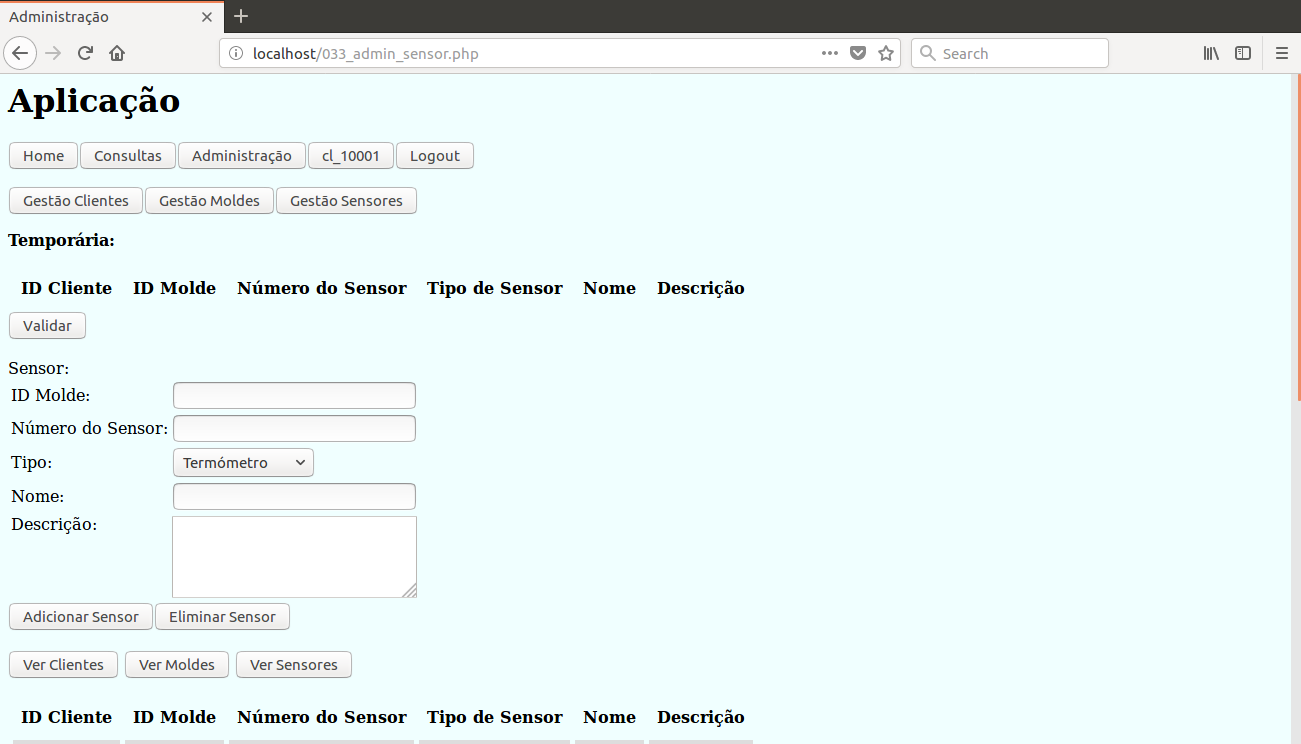
\includegraphics[width=0.8\textwidth]{administracao06} % Include the image placeholder.png
			\caption{Área de Gestão de Sensores}
			\label{fig:admin10}
	\end{figure}
Quando a informação dos moldes e sensores estiver completa o botão Validar tenta registar os valores presentes na base de dados temporária local nas bases de dados central e local. Se a ação não executar com sucesso é retornado um erro \textit{MySQL} de forma a informar o utilizador. Se a ação executar com sucesso a base de dados temporária local é limpa e os valores são registados permanentemente nas bases de dados central e local, como representado nas Figuras \ref{fig:admin12} e \ref{fig:admin13}.\\
Depois de inseridos, moldes e sensores, não podem ser eliminados via aplicação. Esta opção foi removida da aplicação para evitar erros, dado que apagar um molde em funcionamento faz com que se percam novos registos.
\begin{figure}[H]
	\centering
	\begin{minipage}{.5\textwidth}
		\begin{center}
			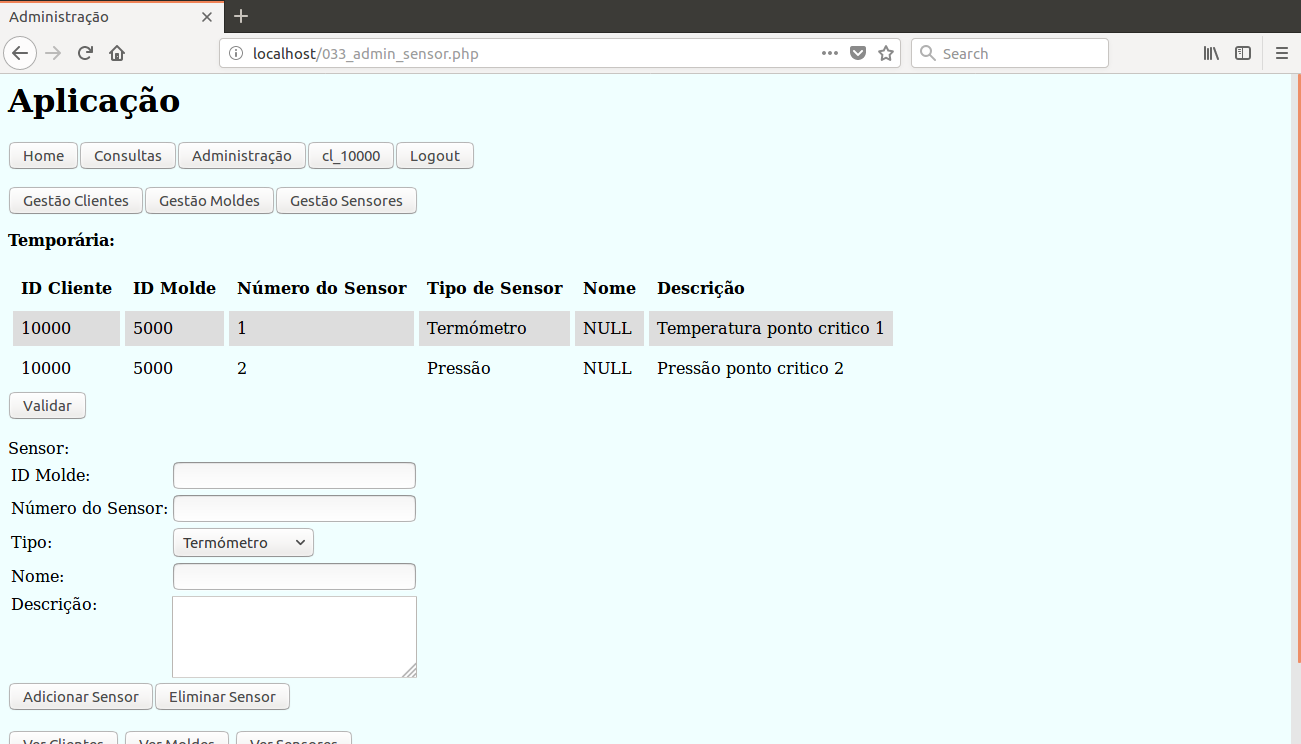
\includegraphics[width=0.9\textwidth]{administracao07} % Include the image placeholder.png
			\subcaption{Dados antes de serem validados}
			\label{fig:admin12}
		\end{center}
	\end{minipage}%
	\begin{minipage}{.5\textwidth}
		\begin{center}
			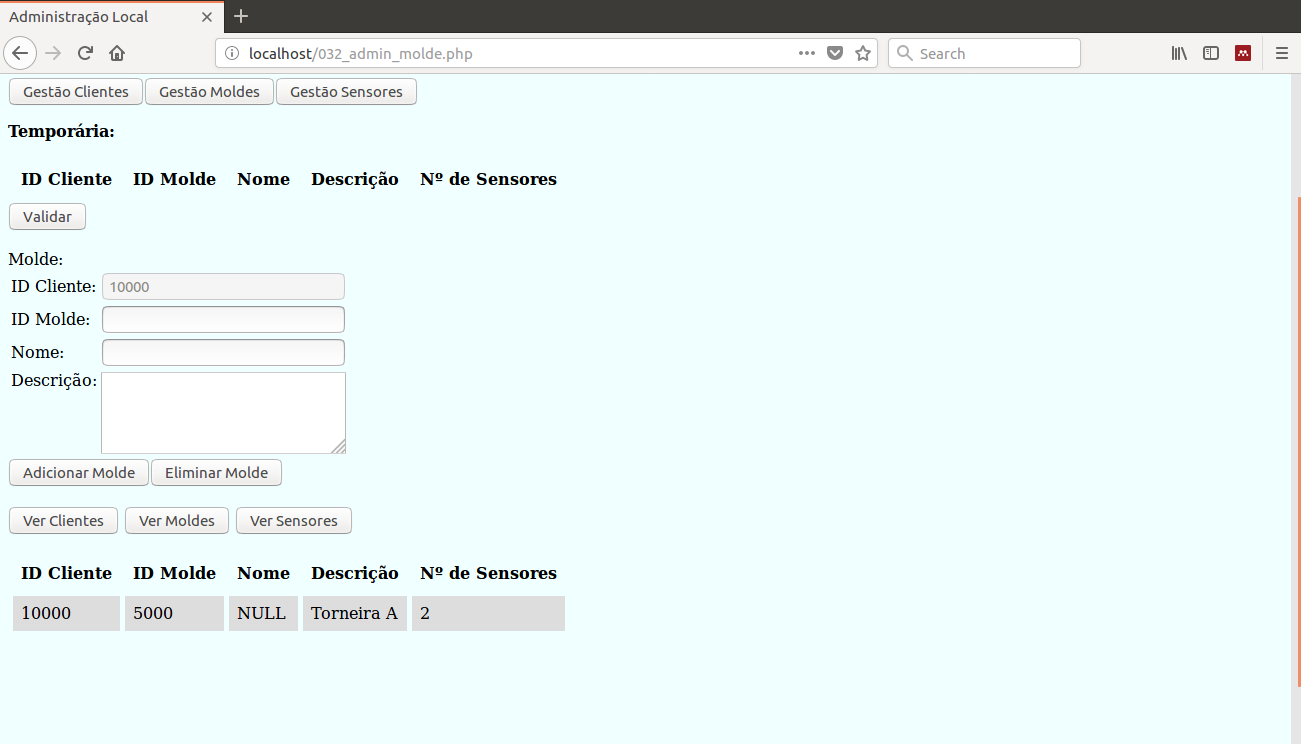
\includegraphics[width=0.9\textwidth]{administracao08} % Include the image placeholder.png
			\subcaption{Dados após serem validados}
			\label{fig:admin13}
		\end{center}
	\end{minipage}
	\caption{Função do botão Validar, onde os valores da base de dados temporária local são transferidos de forma permanente para as bases de dados central e local}
	\label{fig:admin11}
\end{figure}
Voltando a área de Gestão de Clientes, após a conexão local, desbloqueia-se uma nova funcionalidade como demonstra a \autoref{fig:admin7}. O botão Atualizar permite reiniciar o programa de transferência de valores para que este atualize o número de clientes. Com o comando:
\begin{lstlisting}[language = bash]
	ps ax | grep transferencia
\end{lstlisting}
Obtém-se os números de processo dos programas que estão a transferir valores. Estes valores são armazenados na variável @pids. Para terminar os programas utiliza-se o seguinte comando:
\begin{lstlisting}[language = bash]
	kill -2 @pids
\end{lstlisting}
A opção -2 permite enviar para o processo escolhido o sinal SIGINT que é o sinal esperado pelo programa para que este termine as suas rotinas antes de encerrar. Para iniciar novamente o comando usar:
\begin{lstlisting}[language = bash]
	~/path/transferencia
\end{lstlisting}
É necessário garantir permissões ao servidor \textit{Apache} no sistema central para que este possa executar estes comandos.
\newpage
\begin{figure}[H]
	\centering
			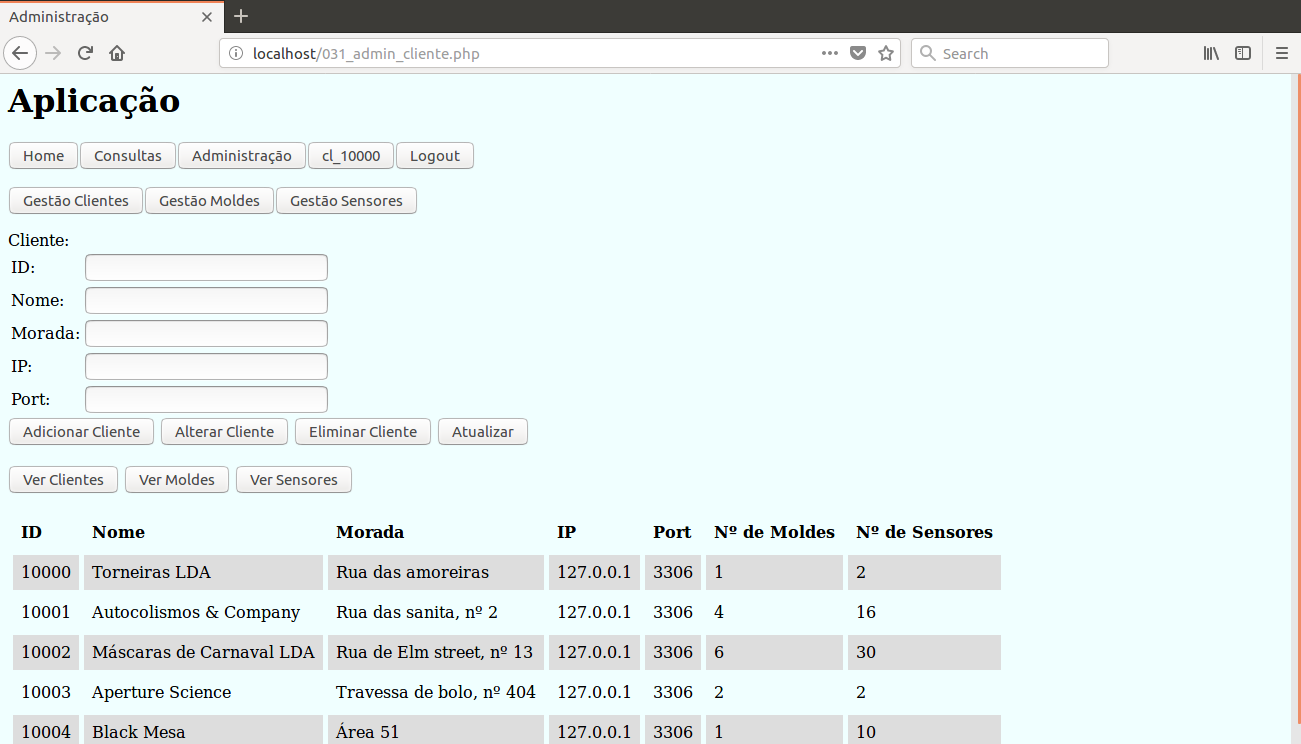
\includegraphics[width=0.9\textwidth]{administracao04} % Include the image placeholder.png
	\caption{Área de Gestão de Clientes após conexão local onde se visualiza o botão Atualizar}
	\label{fig:admin7}
\end{figure}
Nas várias áreas de gestão existem os botões Ver Clientes, Ver Moldes e Ver Sensores que executam respetivamente as \textit{queries}:
\begin{lstlisting}[language = SQL]
	SELECT cl_ID, cl_nome, cl_morada, cl_IP, cl_port,
	COUNT(DISTINCT m_ID), COUNT(DISTINCT s_IDMolde, s_num)
	FROM clientes
	LEFT OUTER JOIN moldes ON cl_ID = m_IDCliente
	LEFT OUTER JOIN sensores ON m_ID = s_IDMolde
	GROUP BY cl_ID
	ORDER BY cl_ID
	
	SELECT m_IDCliente, m_ID, m_nome, m_descricao,
	COUNT(DISTINCT s_IDMolde, s_num)
	FROM clientes
	INNER JOIN moldes ON cl_ID = m_IDCliente
	LEFT OUTER JOIN sensores ON m_ID = s_IDMolde
	GROUP BY m_ID
	ORDER BY m_IDCliente, m_ID
	
	SELECT m_IDCliente, s_IDMolde, s_num, tipo_nome,
	s_nome, s_descricao
	FROM moldes
	INNER JOIN sensores ON m_ID = s_IDMolde
	INNER JOIN tipo ON s_tipo = tipo_id
	ORDER BY m_IDCliente, s_IDMolde, s_num
\end{lstlisting}
Estas fornecem algumas informações contextuais para facilitar a navegação do utilizador.

\subsection{Conexão local}
\label{subchap:local}
	\begin{figure}[H]
		\centering
			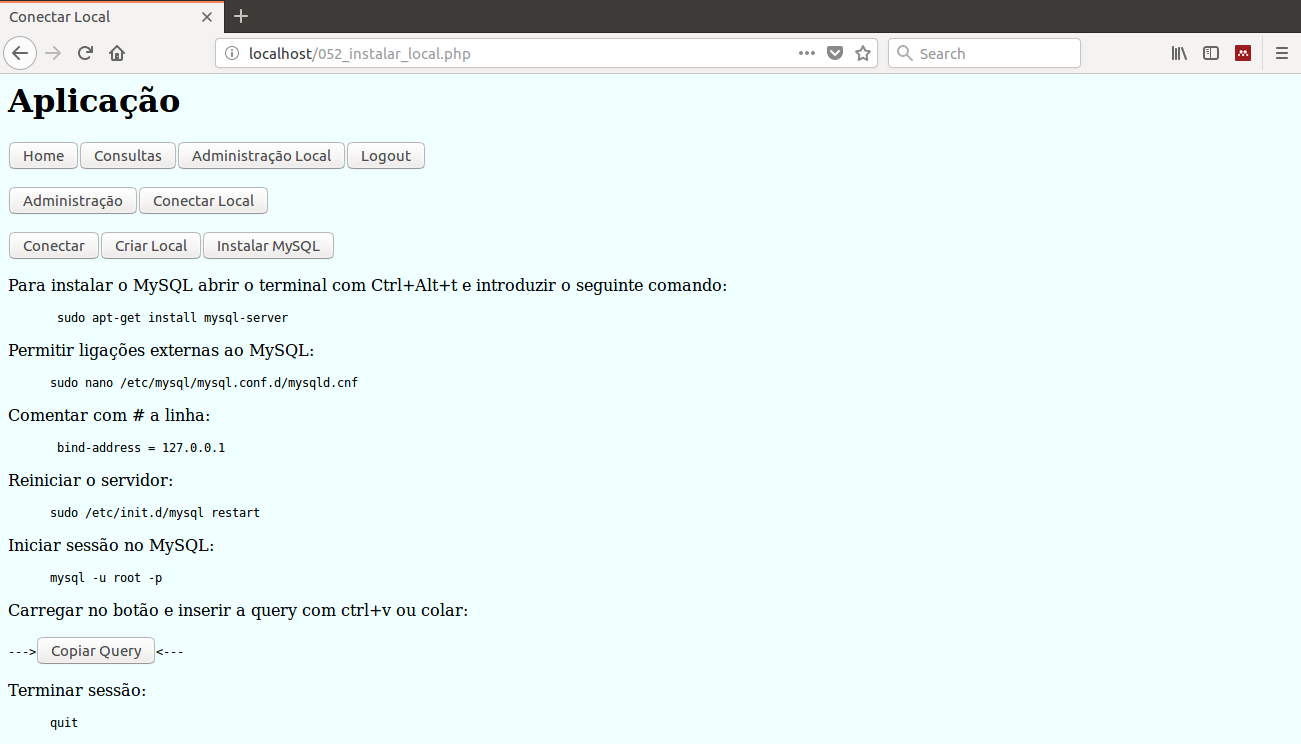
\includegraphics[width=0.9\textwidth]{local01} % Include the image placeholder.png
			\caption{Área Conectar Local onde se visualiza as bases de dados instaladas no sistema}
			\label{fig:local1}
	\end{figure}
A área de Conectar Local na \autoref{fig:local1} permite realizar uma conexão à base de dados local no servidor do cliente. Com recurso à \textit{query}:
\begin{lstlisting}[language = SQL]
	SHOW DATABASES
\end{lstlisting}
Obtém-se todas as bases de dados instaladas no servidor local. Do ponto de vista prático, cada cliente só terá uma base de dados local mas, para efeitos de desenvolvimento do projeto adotou-se esta vertente.
O botão Conectar inicia sessão na base de dados local escolhida e redireciona o utilizador para a página principal como se observar na \autoref{fig:local4}. O botão Desconectar termina esta sessão e redireciona o utilizador também, para a página principal.
\newpage
\begin{figure}[H]
	\begin{center}
		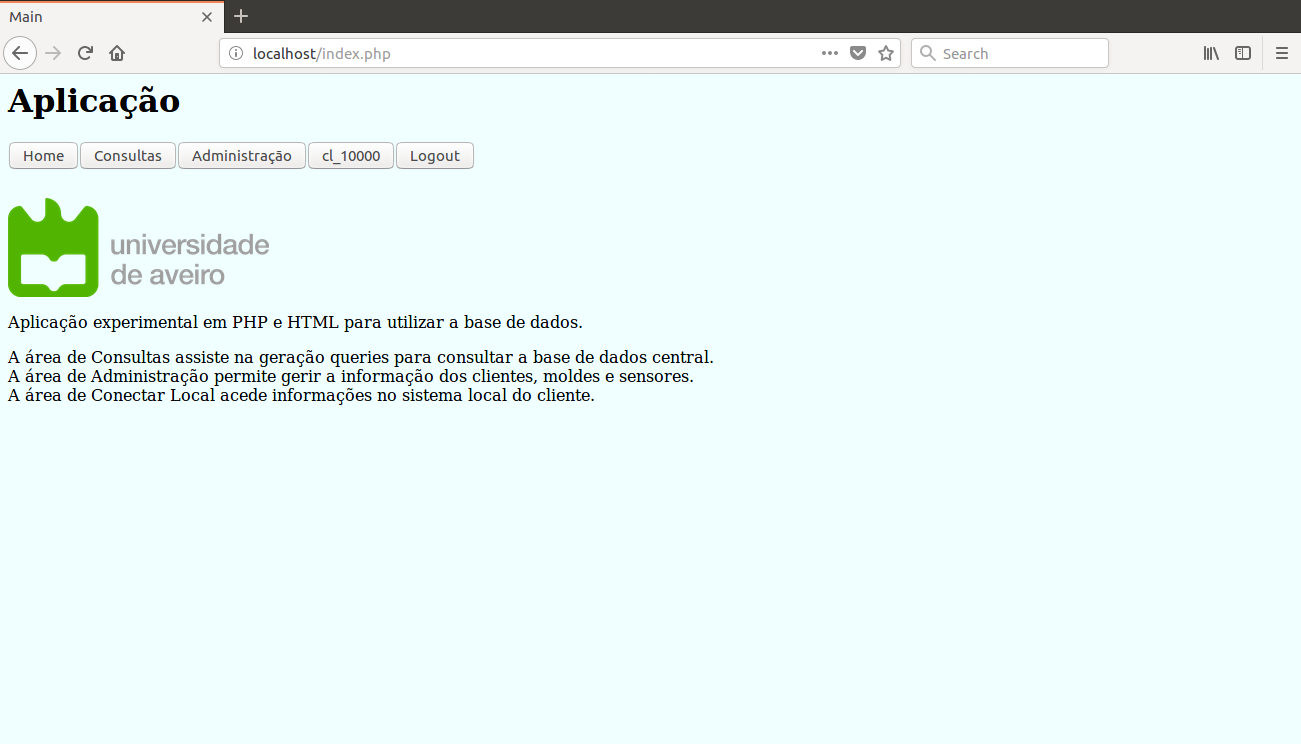
\includegraphics[width=0.9\textwidth]{main03} % Include the image placeholder.png
		\caption{\textit{Main} com conexão local}
		\label{fig:local4}
	\end{center}
\end{figure}
	\begin{figure}[H]
		\centering
		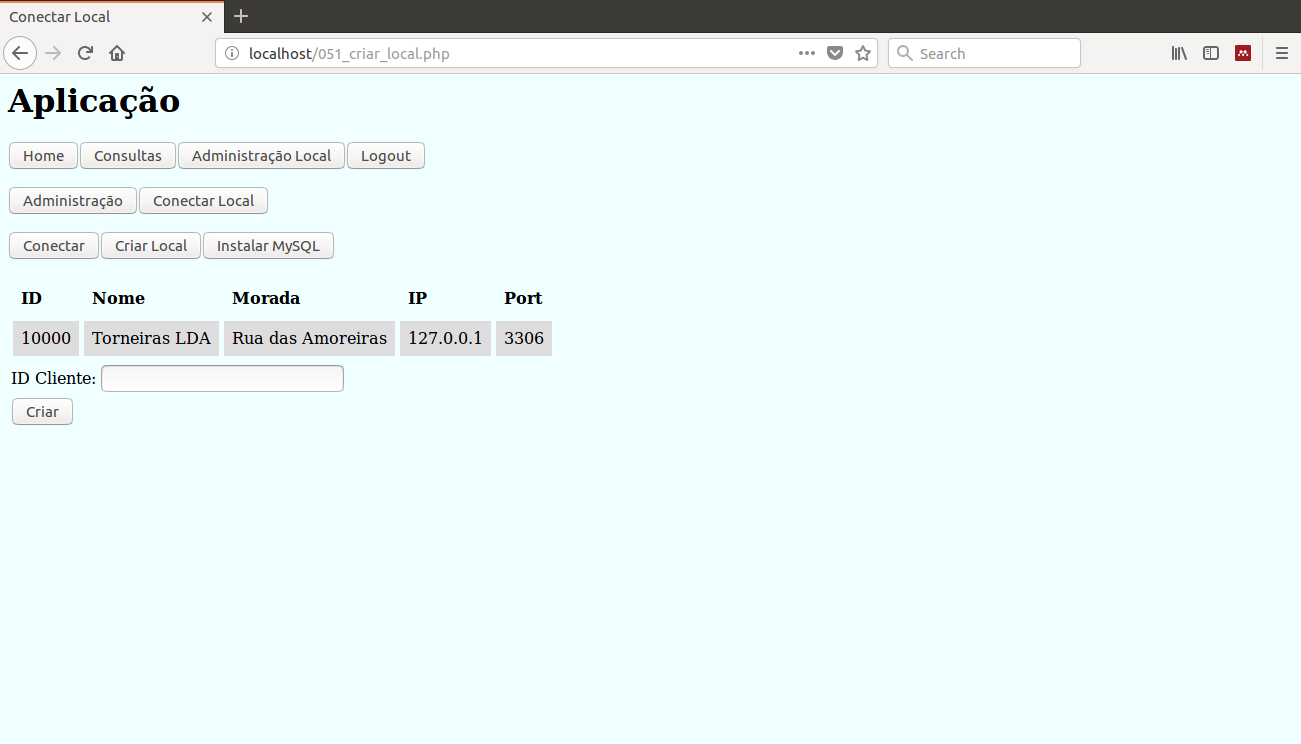
\includegraphics[width=0.9\textwidth]{local02} % Include the image placeholder.png
		\caption{Área Criar Local cria a base de dados para o cliente selecionado no sistema em que se acede a aplicação}
		\label{fig:local2}
	\end{figure}
A área Criar Local na \autoref{fig:local2} permite instalar uma base de dados para um novo cliente. São considerados novos clientes todos os que não tenham moldes associados a si, esta informação obtém-se com a \textit{query}:
\newpage
\begin{lstlisting}[language = SQL]
	SELECT cl_ID, cl_nome, cl_morada, cl_IP, cl_port
	FROM
		(SELECT cl_ID, cl_nome, cl_morada, cl_IP, cl_port,
		COUNT(DISTINCT m_ID) AS n_moldes
		FROM clientes
		LEFT OUTER JOIN moldes ON cl_ID = m_IDCliente
		GROUP BY cl_ID) AS contagem
	WHERE n_moldes = 0
\end{lstlisting}
Escolhendo um cliente válido o botão Criar cria a base de dados local com as respetivas tabelas e gera ainda as \textit{queries} observadas na \autoref{fig:local5}.
\begin{figure}[H]
	\begin{center}
		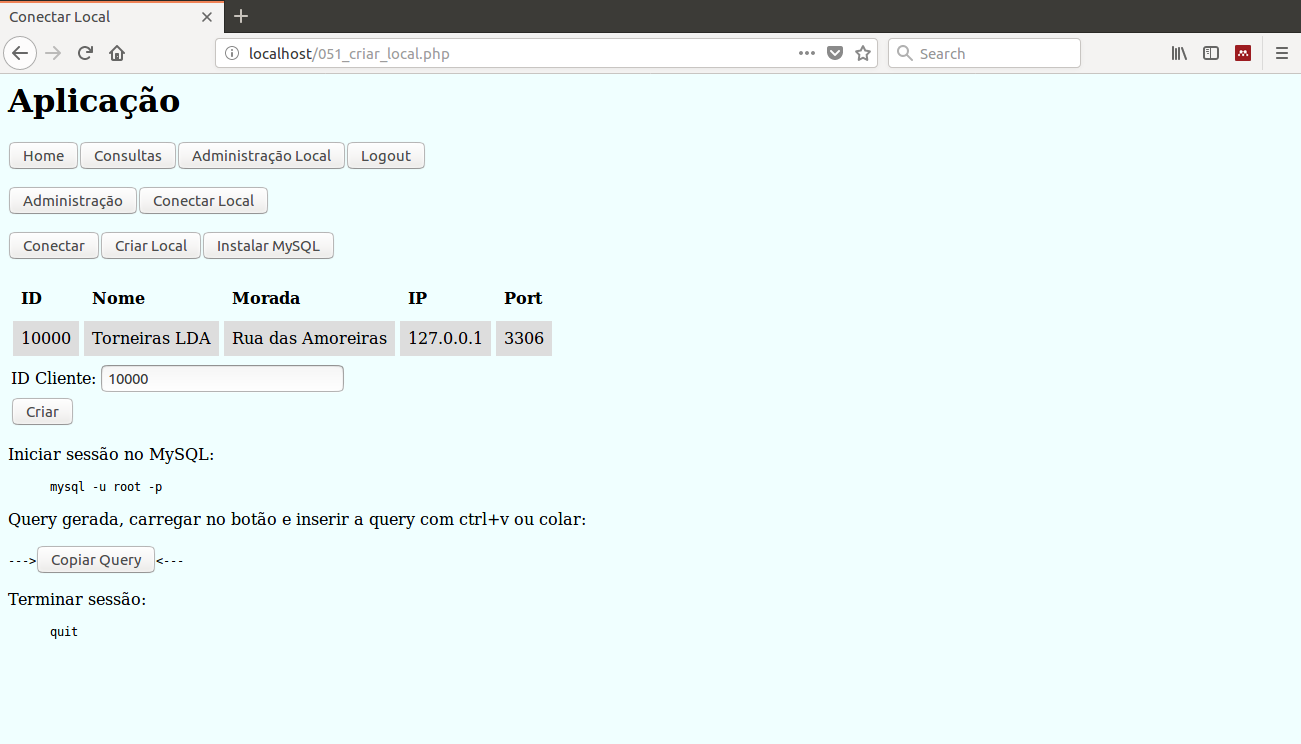
\includegraphics[width=0.9\textwidth]{local03} % Include the image placeholder.png
		\caption{\textit{Queries} geradas para completar a instalação da base de dados no sistema local. Consistem nas permissões para os utilizadores que só podem ser garantidas via \textit{root} bem como informação para completar o sistema de dados}
		\label{fig:local5}
	\end{center}
\end{figure}
\newpage
Terminado a análise das funcionalidades da aplicação com a área de Instalar \textit{MySQL} na \autoref{fig:local3} que contém os passos para instalar o \textit{MySQL} num sistema \textit{Linux}.
\begin{figure}[H]
	\centering
	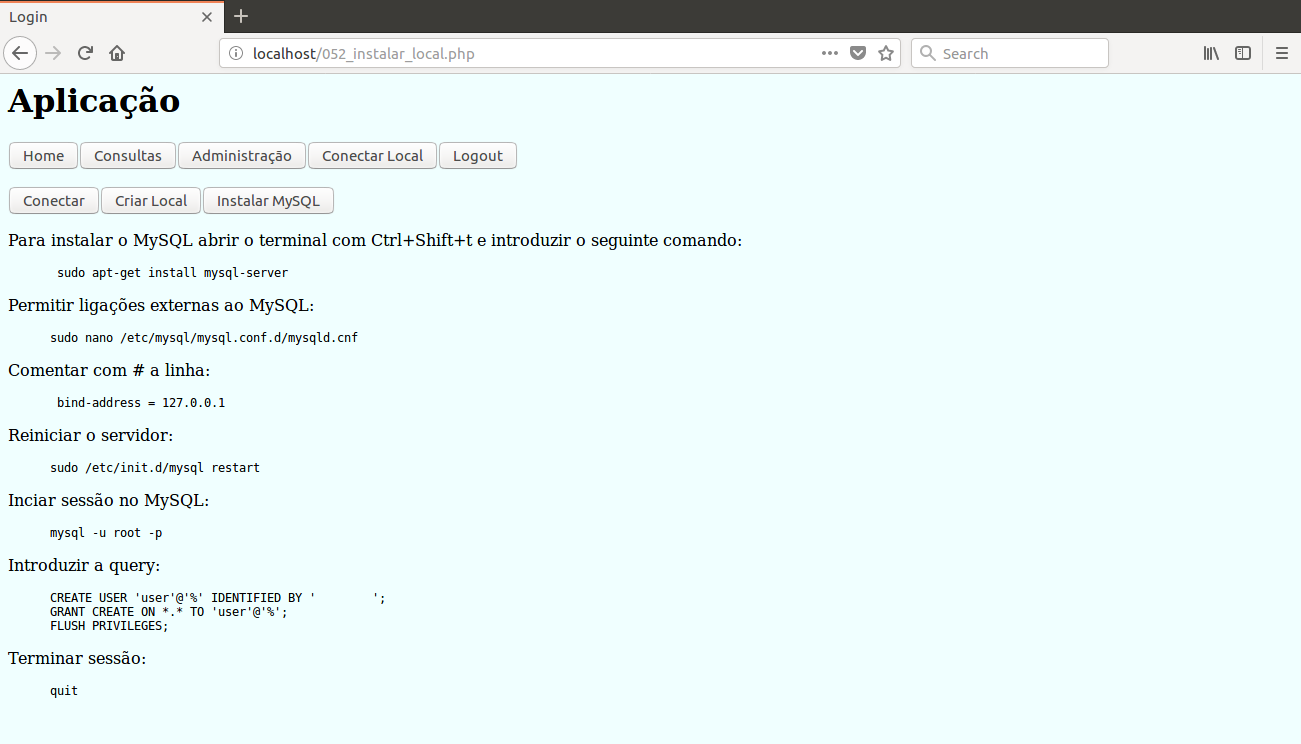
\includegraphics[width=0.9\textwidth]{local04} % Include the image placeholder.png
	\caption{Área Instalar \textit{MySQL} para instalar o \textit{software} com os comandos em \textit{Linux}}
	\label{fig:local3}
\end{figure}

\cleardoublepage
\chapter{Instalação do Sistema}

\cleardoublepage
\chapter{Conclusões}
O desafio proposto consiste em monitorizar sensores remotamente. Para isto definiu-se como objetivos principais desenvolver uma rede de bases de dados e uma aplicação que permitisse interagir com estas. Estes objetivos foram concluídos com sucesso. Este capítulo contém comentários sobre o desempenho da solução desenvolvida e propostas para trabalhos futuros.

\section{Comentários}
\subsection{Infraestrutura de dados}
Em relação à infraestrutura proposta, esta cumpre todos os requisitos propostos de garantir uma transferência segura, confidencial e permanente de valores, criando um histórico dos moldes monitorizados. Os programas desenvolvidos em \textit{C} são simples e funcionais. No entanto, quando estão em funcionamento, o sistema executa-os sem restrições. Isto resulta num elevado consumo do processador e consequente perda de performance do sistema central. Esta perda de performance pode ser por causa do \textit{hardware} utilizado no projeto e a utilização de um sistema devidamente dimensionado para a tarefa em mão pode resolver este problema. Outra solução seria limitar a velocidade de processamento da execução destes programas.\\
Como definido nos objetivos esta não impõe restrições na instrumentação dos moldes. Para introduzir dados nas bases de dados locais pode ser utilizado qualquer sistema operativo e linguagem de programação desde que esta tenha protocolos de comunicação com \textit{MySQL} e gere \textit{queries} do tipo:
\begin{lstlisting}[language = SQL]
	INSERT INTO registos
	VALUES
	(molde, sensor, fase, data_hora, milissegundos, valor);
\end{lstlisting}
Na realidade esta infraestrutura pode ser utilizada em qualquer contexto de monitorização remota de sensores desde que seja desenvolvido um modelo de dados apropriado.

\subsection{Aplicação}
Em relação à aplicação, esta cumpre os objetivos propostos de ser multiplataforma e garantir um acesso remoto à base de dados central, bem como gerir as informações dos clientes, moldes e sensores. No entanto, o facto da aplicação ter sido desenvolvida na totalidade com \textit{PHP} e \textit{HTML}, causa uma perda de performance no servidor central. Isto aconteceu porque, durante o desenvolvimento do projeto, não foi percebido na totalidade o conceito de lado do servidor e lado do cliente. De forma a melhorar o desempenho sugere-se a alteração de algumas funcionalidades desenvolvidas em \textit{PHP} para \textit{JavaScript}, como por exemplo, as conexões às bases de dados que são particularmente pesadas no servidor. A alteração das conexões de \textit{PHP} para \textit{JavaScript} permite também alterar o método de instalação da base de dados local mencionado na \autoref{subchap:local}. Em vez de serem gerados comandos para o utilizador executar no \textit{MySQL} estes podem ser enviados diretamente pela aplicação desde que seja fornecida a \textit{password} para a \textit{root} do sistema como sugerido na \autoref{fig:conclusoes1}.
\begin{figure}[H]
	\begin{center}
		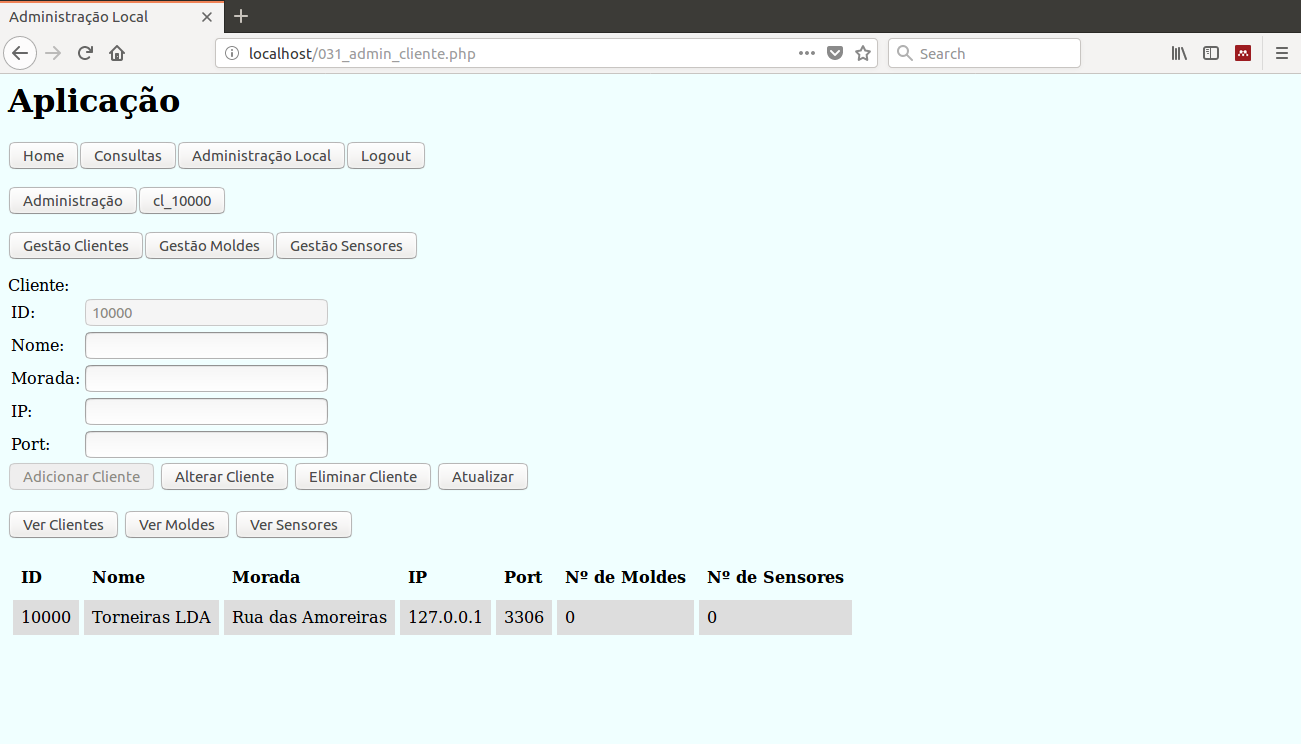
\includegraphics[width=0.9\textwidth]{futuro01} % Include the image placeholder.png
		\caption{Área de Criar Local com criação via \textit{root} em vez de gerar \textit{queries} para o utilizador inserir manualmente no \textit{MySQL}}
		\label{fig:conclusoes1}
	\end{center}
\end{figure}
Além disto é necessário realizar uma revisão de segurança à aplicação. Por exemplo, o botão Atualizar na área Gestão de Clientes que reinicia o programa de transferência de valores através de comandos no terminal. Se as permissões garantidas ao servidor \textit{Apache} não forem bem definidas, pode constituir uma quebra de segurança. Um programador com intenções maliciosas pode acessar o sistema pela aplicação e realizar comandos no terminal de forma a comprometer o sistema. Para isto não acontecer é necessário garantir que o servidor \textit{Apache} só tem permissões sobre o programa de transferência ou então definir um sistema de notificações entre a aplicação e o programa em \textit{C}.\\
Apesar de serem necessários alguns ajustes de forma a melhorar performance, a solução proposta da infraestrutura e aplicação é completamente funcional e pode ser já implementada numa fase experimental.

\section{Trabalhos Futuros}
Quanto à infraestrutura dos dados não foi definido como os sensores dos moldes serão ligados ao servidor local. No desenvolvimento deste projeto assumiu-se que todos os moldes estão ligados diretamente ao sistema local. Se esta proposta não se demonstrar viável é possível, em vez de se ter um servidor local por cliente, ter um servidor local por molde. Esta adaptação irá criar uma maior quantidade de bases de dados locais mas, isto não é problemático, se o modelo de dados e o programa de transferência forem adaptados para o efeito.\\
Quanto à aplicação, sugere-se que após uma apresentação inicial desta à empresa promotora, seja iniciado um processo iterativo de desenvolvimento para escolher e desenvolver novas funcionalidades que possam ser úteis e que não tenham sido abrangidas neste projeto, como por exemplo, a criação de utilizadores baseado no ID de trabalhador demonstrado na \autoref{fig:conclusoes2}. Culminando numa estilização da aplicação para que esta tenha um aspeto mais amigável ao utilizador.
\begin{figure}[H]
	\begin{center}
		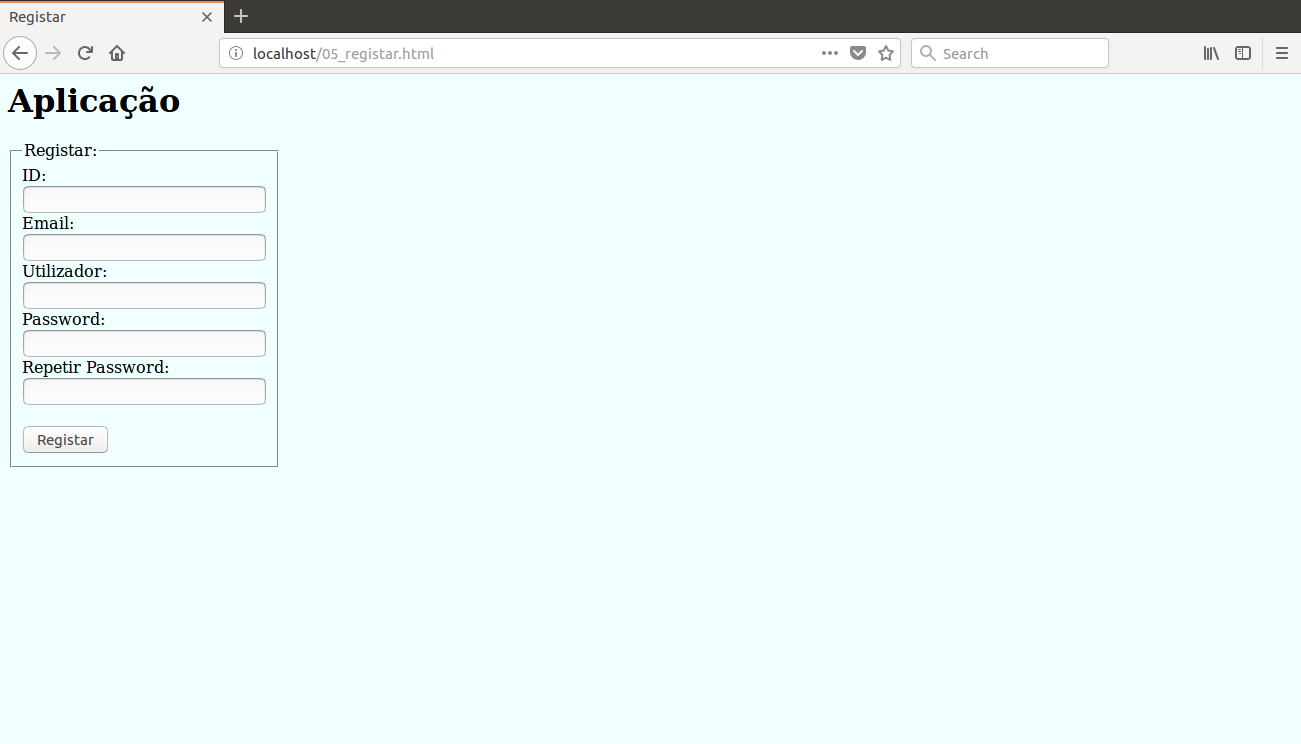
\includegraphics[width=0.9\textwidth]{futuro02} % Include the image placeholder.png
		\caption{Exemplo de área de Registar para criar utilizadores com base no ID de trabalhador e email}
		\label{fig:conclusoes2}
	\end{center}
\end{figure}
\vspace{-.82cm}
Além destas alterações sugere-se a criação de um sistema de notificações e monitorização automático dos moldes. É impossível para um utilizador analisar manualmente milhões de registos de um molde e concluir se este está a funcionar corretamente. Para este efeito criar um programa capaz de correr algoritmos que analisem o comportamento dos moldes. Este programa pode ser desenvolvido em \textit{softwares} mais sofisticados, como por exemplo \textit{MATLAB}, desde que estes tenham protocolos de comunicação com \textit{MySQL}.\looseness=-1\\
A gestão dos \textit{backups} descrita na \autoref{subchap:backups} onde se separa os registos dos moldes em vez de se realizar um \textit{backup} geral foi realizada com este sistema de notificações em mente. Se for necessário, para efeitos de cálculo, que o programa carregue os registos de um molde armazenados em \textit{backups}, este só necessita de carregar a informação do molde que está a ser analisado em vez de ter de carregar a informação de todos os moldes. Este programa deverá correr automaticamente no sistema de forma permanente ou com um temporizador e, no caso de ser necessário, notificar o utilizador via aplicação ou via email.

%
% The bibliography
%
\cleardoublepage
\bibliographystyle{unsrt}
\bibliography{bib/own/molde.bib}

%%\sloppy
%%\printbibliography[prenote=myprenote,title=References]
%\iffalse
%  % Use this is the final version
%  %  unsrt produces numbered entries, sorted by order of citation
%  %  plain produces numbered entries, sorted alphabetically
%  %  other styles are possible (I recommend the harvard package)
%  \bibliographystyle{unsrt}
%  %\bibliographystyle{plain}
%  \bibliography{molde}% replace by the name of name of your .bib file
%\else
%  % An example (the contents of the .bbl file)
%  \begin{thebibliography}{10}
%
%  \bibitem{Eliahou-1-1993-CLBNCL}
%  Shalom Eliahou.
%  \newblock The $3x+1$ problem: New lower bounds on nontrivial cycle lengths.
%  \newblock {\em Discrete Mathematics}, 118(1--3):45--56, 1993.
%
%  \bibitem{Garner-1981-1-OCA}
%  Lynn~E. Garner.
%  \newblock On the collatz $3n+1$ algorithm.
%  \newblock {\em Proceedings of the American Mathematical Society}, 82(1):19--22,
%    May 1981.
%  \end{thebibliography}
%\fi
\cleardoublepage

\end{document}
